\documentclass[10pt,aspectratio=169]{beamer}

\usetheme{default}
\usefonttheme{professionalfonts}

\usepackage[utf8]{inputenc}
\usepackage[T1]{fontenc}
\usepackage{lmodern}
\usepackage{amsmath}
\usepackage{booktabs}
\usepackage{array}
\usepackage{tikz}
\usepackage{listings}
\usepackage{xcolor}
\usepackage{graphicx}
\usepackage{multicol}

\usetikzlibrary{arrows.meta,positioning,shapes.geometric,calc,decorations.pathreplacing,fit,backgrounds,matrix}
\graphicspath{{presentation/assets/}{assets/}{figures/}{../figures/}}

% -------------------------------------------------------------------
% Visual system
% -------------------------------------------------------------------
\definecolor{Navy}{HTML}{071B33}
\definecolor{Ink}{HTML}{17212B}
\definecolor{Muted}{HTML}{5B6773}
\definecolor{Cyan}{HTML}{13A8A8}
\definecolor{Blue}{HTML}{165DFF}
\definecolor{Green}{HTML}{2E7D32}
\definecolor{Orange}{HTML}{F08A24}
\definecolor{Red}{HTML}{B3261E}
\definecolor{Paper}{HTML}{F6F8FB}
\definecolor{Line}{HTML}{D9E1EA}
\definecolor{SoftBlue}{HTML}{EAF2FF}
\definecolor{SoftCyan}{HTML}{E7F8F8}
\definecolor{SoftGreen}{HTML}{ECF6EE}
\definecolor{SoftOrange}{HTML}{FFF2E3}
\definecolor{SoftRed}{HTML}{FCEBEC}

\setbeamercolor{normal text}{fg=Ink,bg=white}
\setbeamercolor{structure}{fg=Blue}
\setbeamercolor{frametitle}{fg=Navy,bg=white}
\setbeamercolor{block title}{fg=white,bg=Navy}
\setbeamercolor{block body}{fg=Ink,bg=Paper}
\setbeamercolor{block title example}{fg=white,bg=Green}
\setbeamercolor{block body example}{fg=Ink,bg=SoftGreen}
\setbeamercolor{block title alerted}{fg=white,bg=Red}
\setbeamercolor{block body alerted}{fg=Ink,bg=SoftRed}

\setbeamertemplate{navigation symbols}{}
\setbeamertemplate{itemize item}{\color{Cyan}$\blacktriangleright$}
\setbeamertemplate{itemize subitem}{\color{Orange}$\bullet$}
\setbeamertemplate{enumerate item}{\color{Blue}\insertenumlabel.}

\newcommand{\sgsmalogo}[1][0.62cm]{
\includegraphics[height=#1]{guidelines_img-001.png}}
\newcommand{\code}[1]{\texttt{\footnotesize #1}}
\newcommand{\smallcode}[1]{\texttt{\scriptsize #1}}
\newcommand{\pill}[2]{%
  \tikz[baseline=(n.base)] \node[rounded corners=8pt,fill=#1!13,draw=#1,inner xsep=6pt,inner ysep=2pt] (n) {\scriptsize\bfseries #2};%
}
\newcommand{\metricbox}[3]{%
  \begin{tikzpicture}
    \node[rounded corners=5pt,draw=#1,fill=#1!9,minimum width=2.7cm,minimum height=1.25cm,align=center] {
      {\Large\bfseries #2}\\[-1mm]{\scriptsize #3}
    };
  \end{tikzpicture}
}
\newcommand{\stagebox}[3]{%
  \tikz[baseline=(n.base)] \node[rounded corners=4pt,draw=#1,fill=#1!9,inner xsep=5pt,inner ysep=3pt,text width=#2,align=center,font=\scriptsize] (n) {#3};%
}

\setbeamertemplate{frametitle}{
  \nointerlineskip
  \begin{beamercolorbox}[wd=\paperwidth,ht=0.86cm,dp=0.16cm,leftskip=0.55cm,rightskip=0.45cm]{frametitle}
    \usebeamerfont{frametitle}\insertframetitle\hfill\raisebox{-0.07cm}{\sgsmalogo[0.54cm]}
  \end{beamercolorbox}
  \vspace{-0.22cm}
  \begin{tikzpicture}[remember picture,overlay]
    \draw[Line,line width=0.4pt] ($(current page.north west)+(0,-0.95cm)$) -- ($(current page.north east)+(0,-0.95cm)$);
    \draw[Cyan,line width=1.8pt] ($(current page.north west)+(0,-0.95cm)$) -- ($(current page.north west)+(.28\paperwidth,-0.95cm)$);
  \end{tikzpicture}
  \vspace{0.12cm}
}

\setbeamertemplate{footline}{
  \leavevmode%
  \begin{tikzpicture}[remember picture,overlay]
    \fill[Line] (current page.south west) rectangle ($(current page.south east)+(0,0.035cm)$);
    \fill[Cyan] (current page.south west) rectangle ($(current page.south west)+(0.26\paperwidth,0.035cm)$);
  \end{tikzpicture}
  \hbox{%
    \begin{beamercolorbox}[wd=.72\paperwidth,ht=2.6ex,dp=1.2ex,leftskip=0.55cm]{author in head/foot}
      \scriptsize\color{Muted} Physics-informed PMU event detection and localization
    \end{beamercolorbox}%
    \begin{beamercolorbox}[wd=.28\paperwidth,ht=2.6ex,dp=1.2ex,rightskip=0.55cm plus1fil]{date in head/foot}
      \scriptsize\color{Muted}\hfill \insertframenumber/\inserttotalframenumber
    \end{beamercolorbox}%
  }%
}
\setbeamercolor{author in head/foot}{bg=white}
\setbeamercolor{date in head/foot}{bg=white}

\lstdefinestyle{sgcode}{
  basicstyle=\ttfamily\scriptsize,
  keywordstyle=\color{Blue}\bfseries,
  commentstyle=\color{Muted},
  stringstyle=\color{Green},
  breaklines=true,
  columns=fullflexible,
  keepspaces=true,
  frame=single,
  rulecolor=\color{Line},
  backgroundcolor=\color{Paper},
  showstringspaces=false
}
\lstset{style=sgcode}

\title[SGSMA final method]{Physics-Informed PMU Event Detection and Localization}
\subtitle{A buildable recipe for the final SGSMA submission method}
\author{SGSMA26 Physics-Informed AD}
\date{30-minute hands-on technical walkthrough}

\begin{document}

% -------------------------------------------------------------------
\begin{frame}[plain,noframenumbering]
  \begin{tikzpicture}[remember picture,overlay]
    \fill[Navy] (current page.south west) rectangle (current page.north east);
    \fill[Blue!18] ($(current page.north east)+(-4.2,0)$) -- (current page.north east) -- (current page.south east) -- ($(current page.south east)+(-1.4,0)$) -- cycle;
    \fill[Cyan] ($(current page.south west)+(0,0)$) rectangle ($(current page.south west)+(0.18\paperwidth,0.08)$);
    \fill[Orange] ($(current page.south west)+(0.18\paperwidth,0)$) rectangle ($(current page.south west)+(0.35\paperwidth,0.08)$);
  \end{tikzpicture}
  \vspace{0.35cm}
  \begin{columns}[T,totalwidth=\textwidth]
  \begin{column}{0.68\textwidth}
    {\color{white}\Huge\bfseries Physics-Informed PMU}\\[-1mm]
    {\color{white}\Huge\bfseries Event Detection}\\[2mm]
    {\color{Cyan}\Large and Localization}\\[8mm]
    {\color{white}\large How the submitted pipeline turns raw PMU data into event and location predictions}\\[8mm]
    \pill{Cyan}{sgms\_extra\_trees\_windowed\_v2}\quad
    \pill{Orange}{30 s windows}\quad
    \pill{Green}{ExtraTrees}
  \end{column}
  \begin{column}{0.27\textwidth}
    \centering
    \vspace{0.2cm}
    
\includegraphics[width=0.95\linewidth]{guidelines_img-001.png}\\[3mm]
    {\color{white}\scriptsize SGSMA 2026 Challenge}
  \end{column}
  \end{columns}
  \vfill
  {\color{white}\small Final variant: \code{base\_v2 + rolling + rls\_kalman + graph\_temporal}}
\end{frame}

% -------------------------------------------------------------------
\begin{frame}{What this tutorial covers}
\small
\begin{columns}[T,totalwidth=\textwidth]
\begin{column}{0.48\textwidth}
\begin{block}{Main story}
\begin{enumerate}
  \item Convert raw PMU waveforms into physics-aware features.
  \item Use a hierarchical ExtraTrees classifier to identify event type.
  \item Route each event to a specialized BUS, LINE, or PMU localizer.
  \item Produce the challenge CSV output at timestamp resolution.
\end{enumerate}
\end{block}
\end{column}
\begin{column}{0.48\textwidth}
\begin{exampleblock}{Hands-on goal}
After this talk, you should be able to reimplement the method from scratch if a new dataset is released during the on-site round.
\end{exampleblock}
\begin{alertblock}{Submission boundary}
The final submitted method was SGMS, not the leaky DeepSeek RAW-tuned variants.
\end{alertblock}
\end{column}
\end{columns}
\end{frame}

% -------------------------------------------------------------------
\begin{frame}{30-minute presentation map}
\small
\centering
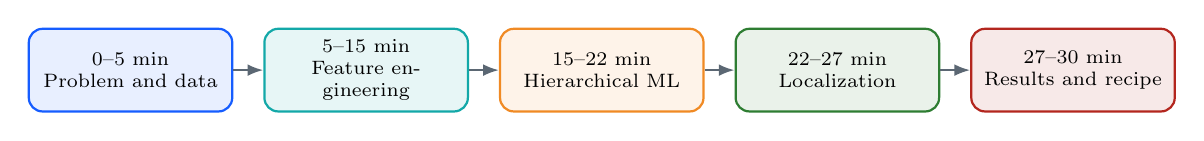
\begin{tikzpicture}[
  boxblue/.style={rounded corners=5pt,draw=Blue,fill=Blue!10,thick,text width=2.35cm,minimum height=1.05cm,align=center,font=\scriptsize},
  boxcyan/.style={rounded corners=5pt,draw=Cyan,fill=Cyan!10,thick,text width=2.35cm,minimum height=1.05cm,align=center,font=\scriptsize},
  boxorange/.style={rounded corners=5pt,draw=Orange,fill=Orange!10,thick,text width=2.35cm,minimum height=1.05cm,align=center,font=\scriptsize},
  boxgreen/.style={rounded corners=5pt,draw=Green,fill=Green!10,thick,text width=2.35cm,minimum height=1.05cm,align=center,font=\scriptsize},
  boxred/.style={rounded corners=5pt,draw=Red,fill=Red!10,thick,text width=2.35cm,minimum height=1.05cm,align=center,font=\scriptsize},
  arrow/.style={-{Latex[length=2mm]},thick,draw=Muted}
]
\node[boxblue] (a) {0--5 min\\Problem and data};
\node[boxcyan,right=0.38cm of a] (b) {5--15 min\\Feature engineering};
\node[boxorange,right=0.38cm of b] (c) {15--22 min\\Hierarchical ML};
\node[boxgreen,right=0.38cm of c] (d) {22--27 min\\Localization};
\node[boxred,right=0.38cm of d] (e) {27--30 min\\Results and recipe};
\draw[arrow] (a) -- (b);
\draw[arrow] (b) -- (c);
\draw[arrow] (c) -- (d);
\draw[arrow] (d) -- (e);
\end{tikzpicture}
\vspace{5mm}
\begin{block}{Backup slides}
Detailed thresholds, artifacts, event-specific recipes, validation commands, and generalization notes are included after the main deck.
\end{block}
\end{frame}

% -------------------------------------------------------------------
\section{Problem and Data}

\begin{frame}[plain]{}
\begin{tikzpicture}[remember picture,overlay]
  \fill[Navy] (current page.south west) rectangle (current page.north east);
  \node[anchor=west] at ($(current page.west)+(0.8,0.6)$) {\color{Cyan}\Large Section 1};
  \node[anchor=west,text width=0.82\paperwidth] at ($(current page.west)+(0.8,-0.15)$) {\color{white}\Huge\bfseries Problem and Data};
  \node[anchor=south east] at ($(current page.south east)+(-0.4,0.35)$) {\sgsmalogo[1.0cm]};
\end{tikzpicture}
\end{frame}

% -------------------------------------------------------------------
\begin{frame}{Challenge task}
\small
\begin{columns}[T,totalwidth=\textwidth]
\begin{column}{0.47\textwidth}
\begin{block}{Input}
Multiple PMU CSV files, usually one per observed bus:
\begin{itemize}
  \item synchronized timestamps,
  \item voltage and current phasors,
  \item frequency and ROCOF,
  \item data-quality indicators.
\end{itemize}
\end{block}
\end{column}
\begin{column}{0.49\textwidth}
\begin{alertblock}{Output}
The submission must generate exactly:
\begin{itemize}
  \item \code{TIMESTAMP}
  \item \code{Bus}
  \item \code{Predicted\_Event}
  \item \code{Predicted\_Location}
\end{itemize}
\end{alertblock}
\end{column}
\end{columns}
\vspace{2mm}
\begin{exampleblock}{Scoring target}
Detection is not enough. The system must also classify the event type and localize its origin or the failed PMU.
\end{exampleblock}
\end{frame}

% -------------------------------------------------------------------
\begin{frame}{The task is three coupled decisions}
\small
\centering
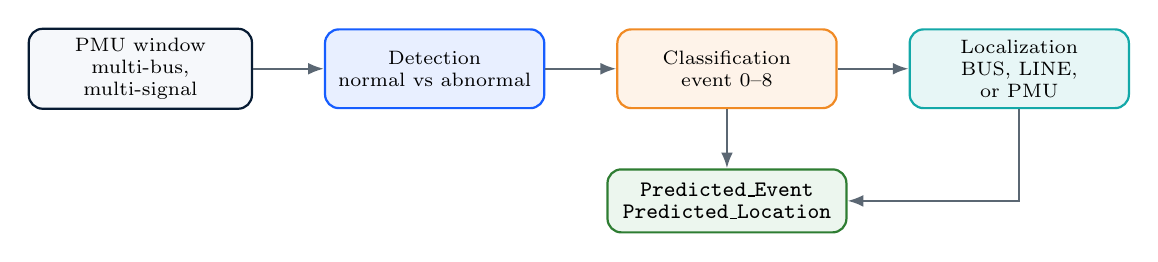
\begin{tikzpicture}[
  node distance=0.5cm and 0.9cm,
  raw/.style={rounded corners=5pt,draw=Navy,fill=Paper,thick,text width=2.6cm,minimum height=1cm,align=center,font=\scriptsize},
  taskblue/.style={rounded corners=5pt,draw=Blue,fill=Blue!10,thick,text width=2.55cm,minimum height=1cm,align=center,font=\scriptsize},
  taskorange/.style={rounded corners=5pt,draw=Orange,fill=Orange!10,thick,text width=2.55cm,minimum height=1cm,align=center,font=\scriptsize},
  taskcyan/.style={rounded corners=5pt,draw=Cyan,fill=Cyan!10,thick,text width=2.55cm,minimum height=1cm,align=center,font=\scriptsize},
  outbox/.style={rounded corners=5pt,draw=Green,fill=SoftGreen,thick,text width=2.8cm,minimum height=0.8cm,align=center,font=\scriptsize},
  arrow/.style={-{Latex[length=2mm]},thick,draw=Muted}
]
\node[raw] (pmu) {PMU window\\multi-bus, multi-signal};
\node[taskblue,right=of pmu] (det) {Detection\\normal vs abnormal};
\node[taskorange,right=of det] (cls) {Classification\\event 0--8};
\node[taskcyan,right=of cls] (loc) {Localization\\BUS, LINE, or PMU};
\node[outbox,below=0.75cm of cls] (csv) {\code{Predicted\_Event}\\\code{Predicted\_Location}};
\draw[arrow] (pmu) -- (det);
\draw[arrow] (det) -- (cls);
\draw[arrow] (cls) -- (loc);
\draw[arrow] (loc) |- (csv);
\draw[arrow] (cls) -- (csv);
\end{tikzpicture}
\vspace{3mm}
\begin{block}{Design consequence}
The pipeline keeps these decisions separate. That is why the final model has a physical classifier, missing/bad-data detectors, and typed localizers instead of one flat classifier.
\end{block}
\end{frame}

% -------------------------------------------------------------------
\begin{frame}{Event labels}
\small
\centering
\begin{tabular}{clp{0.55\textwidth}}
\toprule
\textbf{Label} & \textbf{Name} & \textbf{Physical interpretation}\\
\midrule
0 & normal & No physical disturbance and no major data issue.\\
1 & fault & Strong voltage disturbance, fast derivative, sag or transient.\\
2 & line outage & Current redistribution without fault-level voltage collapse.\\
3 & generation change & Frequency/ROCOF and active-power proxy change.\\
4 & load change & Sustained current and power-consumption change.\\
5 & missing data & Data loss without strong physical evidence.\\
6 & missing + physical & Data loss combined with a real physical event.\\
7 & bad data & One sensor/channel becomes inconsistent with the rest.\\
8 & mixed proxy & Mixed physical signature not cleanly explained by 1--4.\\
\bottomrule
\end{tabular}
\end{frame}

% -------------------------------------------------------------------
\begin{frame}{Raw PMU signals}
\small
\begin{columns}[T,totalwidth=\textwidth]
\begin{column}{0.49\textwidth}
\begin{block}{Electrical measurements}
\begin{tabular}{ll}
\toprule
Group & Columns\\
\midrule
Voltage magnitude & \code{VA\_MAG, VB\_MAG, VC\_MAG}\\
Current magnitude & \code{IA\_MAG, IB\_MAG, IC\_MAG}\\
Voltage angle & \code{VA\_ANG, VB\_ANG, VC\_ANG}\\
Current angle & \code{IA\_ANG, IB\_ANG, IC\_ANG}\\
Dynamics & \code{Freq, ROCOF}\\
\bottomrule
\end{tabular}
\end{block}
\end{column}
\begin{column}{0.47\textwidth}
\begin{block}{Support variables}
\begin{itemize}
  \item \code{TIMESTAMP}: time alignment.
  \item \code{DATA\_PRESENT}: measurement availability.
  \item Bus ID from \code{Bus*.csv}.
  \item IEEE 39-bus topology for graph features.
\end{itemize}
\end{block}
\begin{exampleblock}{Interpretation}
Every feature family is built from a physical question: how large, how fast, how persistent, how coherent, and where in the grid?
\end{exampleblock}
\end{column}
\end{columns}
\end{frame}

% -------------------------------------------------------------------
\begin{frame}{PMU measurement model}
\small
\begin{columns}[T,totalwidth=\textwidth]
\begin{column}{0.50\textwidth}
\begin{block}{Per bus, per phase}
\[
V_{\phi}(t)=|V_{\phi}(t)|e^{j\theta^V_{\phi}(t)},\qquad
I_{\phi}(t)=|I_{\phi}(t)|e^{j\theta^I_{\phi}(t)}
\]
\[
\phi \in \{A,B,C\},\qquad
\dot{f}(t)=\mathrm{ROCOF}(t)
\]
\end{block}
\begin{exampleblock}{What we feed to features}
The extractor uses magnitudes, unwrapped angles, frequency, ROCOF, and data availability. It does not solve a full AC power-flow at inference time.
\end{exampleblock}
\end{column}
\begin{column}{0.46\textwidth}
\centering
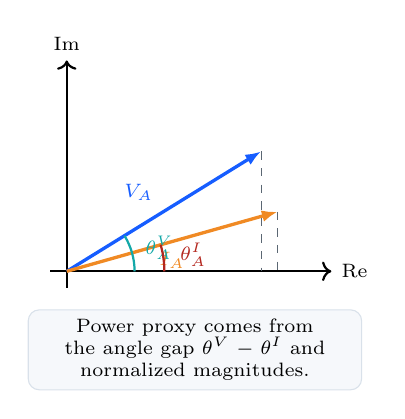
\begin{tikzpicture}[scale=1.05]
  \draw[->,thick] (-0.2,0) -- (3.2,0) node[right]{\scriptsize Re};
  \draw[->,thick] (0,-0.2) -- (0,2.55) node[above]{\scriptsize Im};
  \draw[Blue,very thick,-{Latex[length=2mm]}] (0,0) -- (2.35,1.45) node[midway,above left]{\scriptsize $V_A$};
  \draw[Orange,very thick,-{Latex[length=2mm]}] (0,0) -- (2.55,0.72) node[midway,below]{\scriptsize $I_A$};
  \draw[Cyan,thick] (0.82,0) arc[start angle=0,end angle=31.7,radius=0.82];
  \node[Cyan] at (1.12,0.28) {\scriptsize $\theta^V_A$};
  \draw[Red,thick] (1.18,0) arc[start angle=0,end angle=15.8,radius=1.18];
  \node[Red] at (1.53,0.20) {\scriptsize $\theta^I_A$};
  \draw[Muted,dashed] (2.35,1.45) -- (2.35,0);
  \draw[Muted,dashed] (2.55,0.72) -- (2.55,0);
  \node[rounded corners=4pt,draw=Line,fill=Paper,text width=4.0cm,align=center,font=\scriptsize] at (1.55,-0.95)
  {Power proxy comes from the angle gap $\theta^V-\theta^I$ and normalized magnitudes.};
\end{tikzpicture}
\end{column}
\end{columns}
\end{frame}

% -------------------------------------------------------------------
\begin{frame}{IEEE 39-bus system view}
\small
\begin{columns}[T,totalwidth=\textwidth]
\begin{column}{0.60\textwidth}
\centering
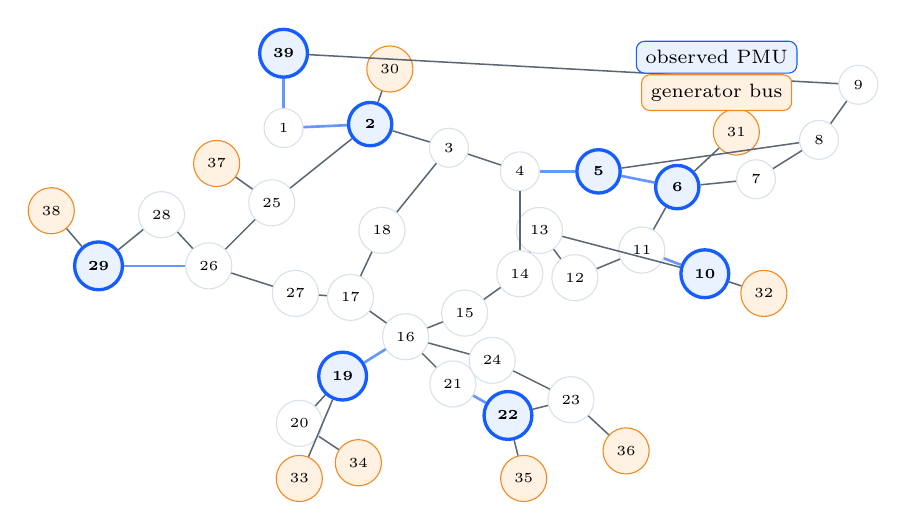
\begin{tikzpicture}[
  bus/.style={circle,draw=Line,fill=white,minimum size=0.44cm,font=\tiny},
  pmu/.style={circle,draw=Blue,fill=SoftBlue,very thick,minimum size=0.55cm,font=\tiny\bfseries},
  gen/.style={circle,draw=Orange,fill=SoftOrange,minimum size=0.46cm,font=\tiny},
  line/.style={draw=Muted,line width=0.55pt},
  obsline/.style={draw=Blue!65,line width=0.95pt}
]
\node[bus] (b1) at (0.0,2.1) {1};
\node[pmu] (b2) at (1.1,2.15) {2};
\node[bus] (b3) at (2.1,1.85) {3};
\node[bus] (b4) at (3.0,1.55) {4};
\node[pmu] (b5) at (4.0,1.55) {5};
\node[pmu] (b6) at (5.0,1.35) {6};
\node[bus] (b7) at (6.0,1.45) {7};
\node[bus] (b8) at (6.8,1.95) {8};
\node[bus] (b9) at (7.3,2.65) {9};
\node[pmu] (b39) at (0.0,3.05) {39};
\node[pmu] (b10) at (5.35,0.25) {10};
\node[bus] (b11) at (4.55,0.55) {11};
\node[bus] (b12) at (3.70,0.20) {12};
\node[bus] (b13) at (3.25,0.80) {13};
\node[bus] (b14) at (3.00,0.25) {14};
\node[bus] (b15) at (2.30,-0.25) {15};
\node[bus] (b16) at (1.55,-0.55) {16};
\node[bus] (b17) at (0.85,-0.05) {17};
\node[bus] (b18) at (1.25,0.80) {18};
\node[pmu] (b19) at (0.75,-1.05) {19};
\node[bus] (b20) at (0.2,-1.65) {20};
\node[bus] (b21) at (2.15,-1.15) {21};
\node[pmu] (b22) at (2.85,-1.55) {22};
\node[bus] (b23) at (3.65,-1.35) {23};
\node[bus] (b24) at (2.65,-0.85) {24};
\node[bus] (b25) at (-0.15,1.15) {25};
\node[bus] (b26) at (-0.95,0.35) {26};
\node[bus] (b27) at (0.15,0.00) {27};
\node[bus] (b28) at (-1.55,1.00) {28};
\node[pmu] (b29) at (-2.35,0.35) {29};
\node[gen] (b30) at (1.35,2.85) {30};
\node[gen] (b31) at (5.75,2.05) {31};
\node[gen] (b32) at (6.10,0.00) {32};
\node[gen] (b33) at (0.20,-2.35) {33};
\node[gen] (b34) at (0.95,-2.15) {34};
\node[gen] (b35) at (3.05,-2.35) {35};
\node[gen] (b36) at (4.35,-2.00) {36};
\node[gen] (b37) at (-0.85,1.65) {37};
\node[gen] (b38) at (-2.95,1.05) {38};
\foreach \a/\b in {b1/b2,b1/b39,b2/b3,b2/b25,b2/b30,b3/b4,b3/b18,b4/b5,b4/b14,b5/b6,b5/b8,b6/b7,b6/b11,b6/b31,b7/b8,b8/b9,b9/b39,b10/b11,b10/b13,b10/b32,b11/b12,b12/b13,b13/b14,b14/b15,b15/b16,b16/b17,b16/b19,b16/b21,b16/b24,b17/b18,b17/b27,b19/b20,b19/b33,b20/b34,b21/b22,b22/b23,b22/b35,b23/b24,b23/b36,b25/b26,b25/b37,b26/b27,b26/b28,b26/b29,b28/b29,b29/b38} {
  \draw[line] (\a) -- (\b);
}
\foreach \a/\b in {b1/b2,b4/b5,b5/b6,b16/b19,b21/b22,b26/b29,b1/b39,b10/b11} {
  \draw[obsline] (\a) -- (\b);
}
\node[rounded corners=3pt,draw=Blue,fill=SoftBlue,font=\scriptsize] at (5.5,3.0) {observed PMU};
\node[rounded corners=3pt,draw=Orange,fill=SoftOrange,font=\scriptsize] at (5.5,2.55) {generator bus};
\end{tikzpicture}
\end{column}
\begin{column}{0.36\textwidth}
\begin{block}{Observed PMUs}
\[
\{2,5,6,10,19,22,29,39\}
\]
\end{block}
\begin{exampleblock}{Electrical reading}
The localizer sees only a sparse set of PMU views. A line or bus event must be inferred from how the disturbance appears across those eight locations.
\end{exampleblock}
\begin{alertblock}{Topology used}
The repo builds electrical distances from the IEEE 39-bus admittance model, not from Euclidean drawing distance.
\end{alertblock}
\end{column}
\end{columns}
\end{frame}

% -------------------------------------------------------------------
\begin{frame}{Topology math: from branches to electrical distance}
\small
\begin{columns}[T,totalwidth=\textwidth]
\begin{column}{0.49\textwidth}
\begin{block}{Admittance and impedance}
\[
Y_{\mathrm{bus}}:\ \text{network admittance matrix}
\]
\[
Z_{\mathrm{bus}}=Y_{\mathrm{bus}}^{+}
\]
\[
d_{ij}^{\mathrm{eff}}=
\left|Z_{ii}+Z_{jj}-Z_{ij}-Z_{ji}\right|
\]
\end{block}
\begin{exampleblock}{Meaning}
Two buses are close if an injection at one bus is expected to have a similar voltage effect at the other.
\end{exampleblock}
\end{column}
\begin{column}{0.47\textwidth}
\centering
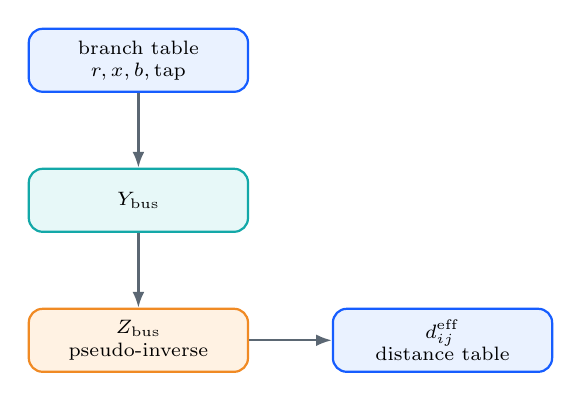
\begin{tikzpicture}[
  node distance=0.95cm,
  box/.style={rounded corners=5pt,draw=Blue,fill=SoftBlue,thick,text width=2.55cm,minimum height=0.8cm,align=center,font=\scriptsize},
  box2/.style={rounded corners=5pt,draw=Cyan,fill=SoftCyan,thick,text width=2.55cm,minimum height=0.8cm,align=center,font=\scriptsize},
  box3/.style={rounded corners=5pt,draw=Orange,fill=SoftOrange,thick,text width=2.55cm,minimum height=0.8cm,align=center,font=\scriptsize},
  arrow/.style={-{Latex[length=2mm]},thick,draw=Muted}
]
\node[box] (br) {branch table\\$r,x,b,\mathrm{tap}$};
\node[box2,below=of br] (y) {$Y_{\mathrm{bus}}$};
\node[box3,below=of y] (z) {$Z_{\mathrm{bus}}$\\pseudo-inverse};
\node[box,right=1.05cm of z] (dist) {$d_{ij}^{\mathrm{eff}}$\\distance table};
\draw[arrow] (br) -- (y);
\draw[arrow] (y) -- (z);
\draw[arrow] (z) -- (dist);
\end{tikzpicture}
\vspace{2mm}
\begin{alertblock}{Where it appears}
Graph-temporal features weight PMU differences by $1/d_{ij}^{\mathrm{eff}}$.
\end{alertblock}
\end{column}
\end{columns}
\end{frame}

% -------------------------------------------------------------------
\begin{frame}{How a case is represented before feature extraction}
\small
\begin{columns}[T,totalwidth=\textwidth]
\begin{column}{0.56\textwidth}
\centering
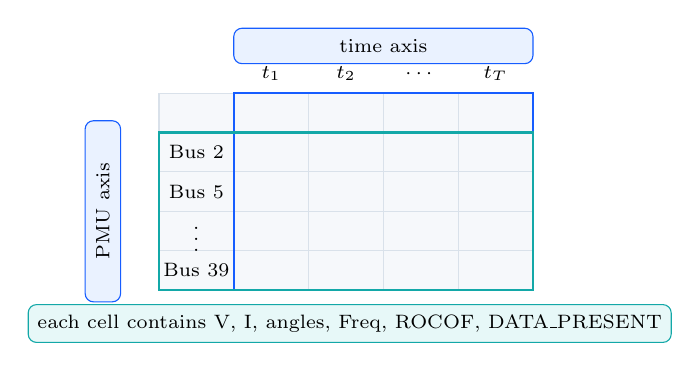
\begin{tikzpicture}[x=0.95cm,y=0.50cm]
  \foreach \r in {0,...,4} {
    \foreach \c in {0,...,4} {
      \draw[Line,fill=Paper] (\c,-\r) rectangle +(1,-1);
    }
  }
  \node[font=\scriptsize] at (1.5,0.5) {$t_1$};
  \node[font=\scriptsize] at (2.5,0.5) {$t_2$};
  \node[font=\scriptsize] at (3.5,0.5) {$\cdots$};
  \node[font=\scriptsize] at (4.5,0.5) {$t_T$};
  \node[font=\scriptsize] at (0.5,-1.5) {Bus 2};
  \node[font=\scriptsize] at (0.5,-2.5) {Bus 5};
  \node[font=\scriptsize] at (0.5,-3.5) {$\vdots$};
  \node[font=\scriptsize] at (0.5,-4.5) {Bus 39};
  \draw[Blue,thick] (1,0) rectangle (5,-5);
  \draw[Cyan,thick] (0,-1) rectangle (5,-5);
  \node[rounded corners=3pt,draw=Blue,fill=SoftBlue,font=\scriptsize,minimum width=3.8cm,minimum height=0.45cm] at (3,1.2) {time axis};
  \node[rounded corners=3pt,draw=Blue,fill=SoftBlue,font=\scriptsize,rotate=90,minimum width=2.3cm,minimum height=0.45cm] at (-0.75,-3) {PMU axis};
  \node[rounded corners=3pt,draw=Cyan,fill=SoftCyan,font=\scriptsize,minimum width=5.3cm,minimum height=0.48cm] at (2.55,-5.85) {each cell contains V, I, angles, Freq, ROCOF, DATA\_PRESENT};
\end{tikzpicture}
\end{column}
\begin{column}{0.40\textwidth}
\begin{block}{The extractor reads a tensor}
Think of one case as a table over PMUs and time. Each table cell has several electrical channels.
\end{block}
\begin{alertblock}{What changes after extraction}
The window becomes one row of engineered features. Models never see the raw tensor directly.
\end{alertblock}
\end{column}
\end{columns}
\end{frame}

% -------------------------------------------------------------------
\begin{frame}{Observed PMUs in the final configuration}
\small
\centering
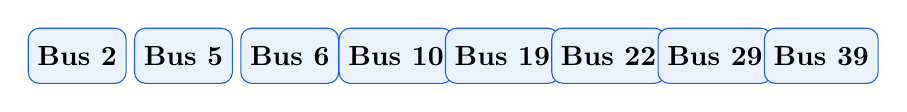
\begin{tikzpicture}[node distance=0.35cm]
\foreach \b [count=\i] in {2,5,6,10,19,22,29,39} {
  \node[rounded corners=4pt,draw=Blue,fill=SoftBlue,minimum width=1.2cm,minimum height=0.7cm] at ({(\i-1)*1.35},0) {\bfseries Bus \b};
}
\end{tikzpicture}
\vspace{5mm}
\begin{block}{Why PMU placement matters}
Localization relies on spatial fingerprints. A disturbance near a bus or line affects nearby PMUs more strongly and often earlier than remote PMUs.
\end{block}
\begin{alertblock}{Generalization note}
The runtime discovers PMU files from \code{Bus*.csv}; it does not hardcode RAW0001 placement in the submitted path.
\end{alertblock}
\end{frame}

% -------------------------------------------------------------------
\begin{frame}{Final runtime route}
\small
\begin{columns}[T,totalwidth=\textwidth]
\begin{column}{0.47\textwidth}
\begin{block}{Entrypoint}
\code{python main.py --input-dir <folder> --output <csv>}
\end{block}
\begin{block}{Active route}
\begin{itemize}
  \item \code{model = sgms\_extra\_trees\_windowed\_v2}
  \item \code{route = ml\_windowed}
  \item \code{window\_seconds = 30}
\end{itemize}
\end{block}
\end{column}
\begin{column}{0.49\textwidth}
\begin{exampleblock}{Call chain}
\code{main.py}\\
$\rightarrow$ \code{src/models/hybrid\_submission.py}\\
$\rightarrow$ \code{src/data\_factory/final\_model.py}
\end{exampleblock}
\begin{alertblock}{Fallback}
A bus-agnostic physics runtime remains only as a missing-bundle fallback.
\end{alertblock}
\end{column}
\end{columns}
\end{frame}

% -------------------------------------------------------------------
\begin{frame}{End-to-end method at a glance}
\centering
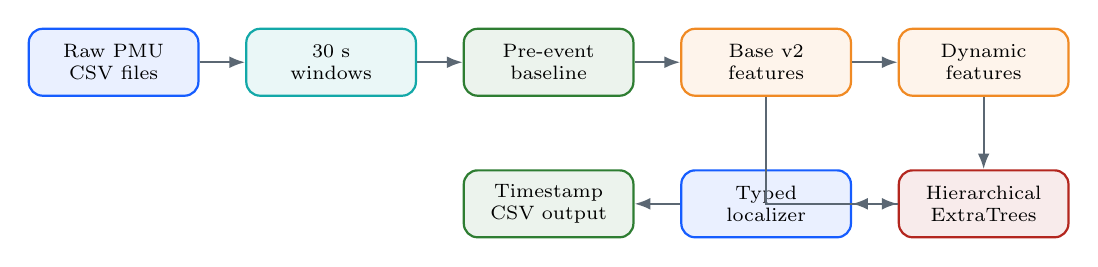
\begin{tikzpicture}[
  node distance=0.58cm,
  boxblue/.style={rounded corners=5pt,draw=Blue,fill=Blue!9,thick,text width=1.92cm,minimum height=0.85cm,align=center,font=\scriptsize},
  boxcyan/.style={rounded corners=5pt,draw=Cyan,fill=Cyan!9,thick,text width=1.92cm,minimum height=0.85cm,align=center,font=\scriptsize},
  boxgreen/.style={rounded corners=5pt,draw=Green,fill=Green!9,thick,text width=1.92cm,minimum height=0.85cm,align=center,font=\scriptsize},
  boxorange/.style={rounded corners=5pt,draw=Orange,fill=Orange!9,thick,text width=1.92cm,minimum height=0.85cm,align=center,font=\scriptsize},
  boxred/.style={rounded corners=5pt,draw=Red,fill=Red!9,thick,text width=1.92cm,minimum height=0.85cm,align=center,font=\scriptsize},
  arrow/.style={-{Latex[length=2mm]},thick,draw=Muted}
]
\node[boxblue] (raw) {Raw PMU\\CSV files};
\node[boxcyan,right=of raw] (win) {30 s\\windows};
\node[boxgreen,right=of win] (base) {Pre-event\\baseline};
\node[boxorange,right=of base] (feat) {Base v2\\features};
\node[boxorange,right=of feat] (dyn) {Dynamic\\features};
\node[boxred,below=0.92cm of dyn] (clf) {Hierarchical\\ExtraTrees};
\node[boxblue,left=of clf] (loc) {Typed\\localizer};
\node[boxgreen,left=of loc] (csv) {Timestamp\\CSV output};
\draw[arrow] (raw) -- (win);
\draw[arrow] (win) -- (base);
\draw[arrow] (base) -- (feat);
\draw[arrow] (feat) -- (dyn);
\draw[arrow] (dyn) -- (clf);
\draw[arrow] (feat) |- (clf);
\draw[arrow] (clf) -- (loc);
\draw[arrow] (loc) -- (csv);
\end{tikzpicture}
\vspace{3mm}
\begin{block}{Runtime shape}
We convert each PMU window into a physics-aware signature, classify the event with guarded ExtraTrees models, then localize it with event-specific localizers.
\end{block}
\end{frame}

% -------------------------------------------------------------------
\begin{frame}{Window prediction expands back to timestamp rows}
\small
\centering
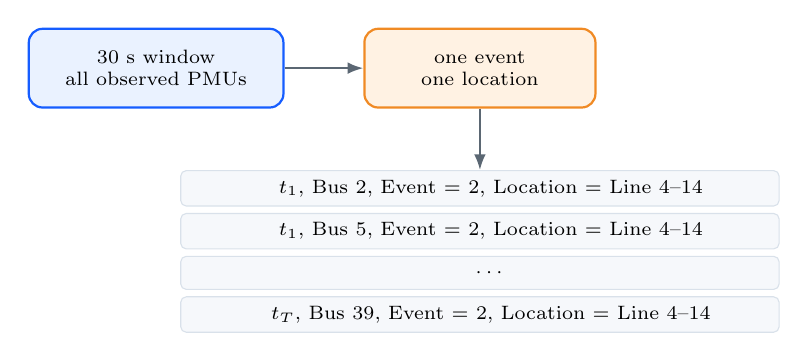
\begin{tikzpicture}[
  node distance=0.7cm,
  win/.style={rounded corners=5pt,draw=Blue,fill=SoftBlue,thick,text width=3.0cm,minimum height=1.0cm,align=center,font=\scriptsize},
  pred/.style={rounded corners=5pt,draw=Orange,fill=SoftOrange,thick,text width=2.7cm,minimum height=1.0cm,align=center,font=\scriptsize},
  row/.style={rounded corners=2pt,draw=Line,fill=Paper,minimum width=7.6cm,minimum height=0.42cm,align=left,font=\scriptsize},
  arrow/.style={-{Latex[length=2mm]},thick,draw=Muted}
]
\node[win] (w) {30 s window\\all observed PMUs};
\node[pred,right=1.0cm of w] (p) {one event\\one location};
\node[row,below=0.78cm of p] (r1) {\quad $t_1$, Bus 2, Event = 2, Location = Line 4--14};
\node[row,below=0.08cm of r1] (r2) {\quad $t_1$, Bus 5, Event = 2, Location = Line 4--14};
\node[row,below=0.08cm of r2] (r3) {\quad $\cdots$};
\node[row,below=0.08cm of r3] (r4) {\quad $t_T$, Bus 39, Event = 2, Location = Line 4--14};
\draw[arrow] (w) -- (p);
\draw[arrow] (p) -- (r1);
\end{tikzpicture}
\vspace{2mm}
\begin{block}{Submission contract}
The official CSV is timestamp-aligned even though the decision is made at the window level.
\end{block}
\end{frame}

% -------------------------------------------------------------------
\section{Windowing and Baseline}

\begin{frame}[plain]{}
\begin{tikzpicture}[remember picture,overlay]
  \fill[Navy] (current page.south west) rectangle (current page.north east);
  \node[anchor=west] at ($(current page.west)+(0.8,0.6)$) {\color{Cyan}\Large Section 2};
  \node[anchor=west,text width=0.82\paperwidth] at ($(current page.west)+(0.8,-0.15)$) {\color{white}\Huge\bfseries Windowing and Baseline};
  \node[anchor=south east] at ($(current page.south east)+(-0.4,0.35)$) {\sgsmalogo[1.0cm]};
\end{tikzpicture}
\end{frame}

% -------------------------------------------------------------------
\begin{frame}{Why a 30-second window?}
\small
\begin{columns}[T,totalwidth=\textwidth]
\begin{column}{0.55\textwidth}
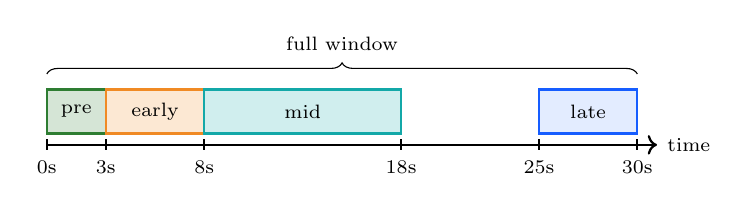
\begin{tikzpicture}[x=0.25cm,y=0.9cm]
  \draw[->,thick] (0,0) -- (31,0) node[right]{\scriptsize time};
  \foreach \x/\txt in {0/0s,3/3s,8/8s,18/18s,25/25s,30/30s} {
    \draw[thick] (\x,0.08) -- (\x,-0.08) node[below]{\scriptsize \txt};
  }
  \fill[Green!20] (0,0.16) rectangle (3,0.78);
  \fill[Orange!20] (3,0.16) rectangle (8,0.78);
  \fill[Cyan!20] (8,0.16) rectangle (18,0.78);
  \fill[Blue!12] (25,0.16) rectangle (30,0.78);
  \draw[Green,thick] (0,0.16) rectangle (3,0.78);
  \draw[Orange,thick] (3,0.16) rectangle (8,0.78);
  \draw[Cyan,thick] (8,0.16) rectangle (18,0.78);
  \draw[Blue,thick] (25,0.16) rectangle (30,0.78);
  \node at (1.5,0.47) {\scriptsize pre};
  \node at (5.5,0.47) {\scriptsize early};
  \node at (13,0.47) {\scriptsize mid};
  \node at (27.5,0.47) {\scriptsize late};
  \draw[decorate,decoration={brace,amplitude=4pt}] (0,1.0) -- node[above=5pt]{\scriptsize full window} (30,1.0);
\end{tikzpicture}
\end{column}
\begin{column}{0.41\textwidth}
\begin{block}{Reasoning}
\begin{itemize}
  \item One sample is too noisy.
  \item A fault has onset and transient.
  \item Load/generation changes are often slower.
  \item Missing data needs run-length evidence.
\end{itemize}
\end{block}
\end{column}
\end{columns}
\vspace{1mm}
\begin{exampleblock}{Implementation}
The model predicts once per window and replicates the window prediction to all required timestamp/bus rows.
\end{exampleblock}
\end{frame}

% -------------------------------------------------------------------
\begin{frame}{Temporal segments}
\small
\centering
\begin{tabular}{lp{0.27\textwidth}p{0.44\textwidth}}
\toprule
\textbf{Segment} & \textbf{Time span} & \textbf{Why it exists}\\
\midrule
pre & first 3 seconds & Estimate normal operating point.\\
early & 3--8 seconds & Capture onset and fast transient.\\
mid & 8--18 seconds & Capture stabilization and oscillation.\\
late & last 5 seconds & Capture persistent post-event level.\\
full & full 30 seconds & Capture total severity and duration.\\
\bottomrule
\end{tabular}
\vspace{3mm}
\begin{alertblock}{Window reading}
The same signal can mean different things depending on when it changes. Timing is part of the physics.
\end{alertblock}
\end{frame}

% -------------------------------------------------------------------
\begin{frame}{Window segmentation math}
\small
\begin{columns}[T,totalwidth=\textwidth]
\begin{column}{0.52\textwidth}
\begin{block}{Given one 30-second window}
\[
t_0=\min(t),\qquad t_1=\max(t),\qquad t_p=t_0+3
\]
\[
\mathcal{T}_{pre}=\{t:t\le t_p\}
\]
\[
\mathcal{T}_{early}=\{t:t_p<t\le t_p+5\}
\]
\[
\mathcal{T}_{mid}=\{t:t_p+5<t\le t_p+15\}
\]
\[
\mathcal{T}_{late}=\{t:t\ge \max(t_p,t_1-5)\}
\]
\end{block}
\end{column}
\begin{column}{0.44\textwidth}
\centering
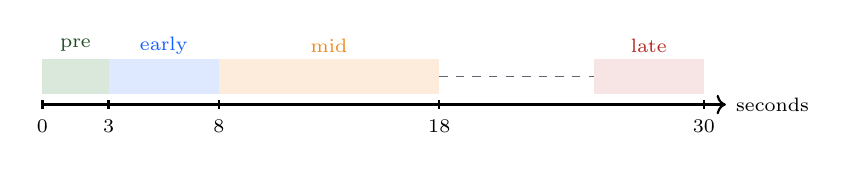
\begin{tikzpicture}[x=0.28cm,y=0.75cm]
  \draw[->,thick] (0,0) -- (31,0) node[right]{\scriptsize seconds};
  \foreach \x/\lab in {0/0,3/3,8/8,18/18,30/30} {
    \draw[thick] (\x,0.08) -- (\x,-0.08) node[below]{\scriptsize \lab};
  }
  \fill[Green!18] (0,0.18) rectangle (3,0.78);
  \fill[Blue!14] (3,0.18) rectangle (8,0.78);
  \fill[Orange!16] (8,0.18) rectangle (18,0.78);
  \fill[Red!12] (25,0.18) rectangle (30,0.78);
  \node[Green!60!black] at (1.5,1.0) {\scriptsize pre};
  \node[Blue] at (5.5,1.0) {\scriptsize early};
  \node[Orange] at (13,1.0) {\scriptsize mid};
  \node[Red] at (27.5,1.0) {\scriptsize late};
  \draw[Muted,dashed] (18,0.48) -- (25,0.48);
\end{tikzpicture}
\vspace{3mm}
\begin{exampleblock}{Why this matters}
Event labels are window labels, but electrical signatures are time-shaped. These masks let us compare the same signal before and after the disturbance.
\end{exampleblock}
\end{column}
\end{columns}
\end{frame}

% -------------------------------------------------------------------
\begin{frame}{Pre-event baseline}
\small
\begin{block}{Baseline per PMU and signal}
\[
b_x = \mathrm{median}\left(x(t),\ t \in \mathrm{pre}\right)
\]
\end{block}
\begin{columns}[T,totalwidth=\textwidth]
\begin{column}{0.47\textwidth}
\begin{exampleblock}{Magnitude normalization}
\[
x_{\mathrm{pu}}(t) = \frac{x(t)}{b_x + \epsilon}
\]
\[
\Delta x(t) = x(t) - b_x
\]
\end{exampleblock}
\end{column}
\begin{column}{0.49\textwidth}
\begin{alertblock}{Angle handling}
Angles are unwrapped before computing differences:
\[
\theta_{\mathrm{clean}} = \mathrm{unwrap}(\theta)
\]
This avoids artificial jumps near the angle boundary.
\end{alertblock}
\end{column}
\end{columns}
\end{frame}

% -------------------------------------------------------------------
\begin{frame}{Baseline and robust scale are computed locally}
\small
\begin{columns}[T,totalwidth=\textwidth]
\begin{column}{0.50\textwidth}
\begin{block}{For each bus $b$ and signal $s$}
\[
m_{b,s}=\mathrm{median}_{t\in \mathcal{T}_{pre}} x_{b,s}(t)
\]
\[
\tilde{x}_{b,s}(t)=x_{b,s}(t)-m_{b,s}
\]
\[
\sigma^{rob}_{b,s}=1.4826\cdot
\mathrm{median}_{t\in \mathcal{T}_{pre}}
\left|x_{b,s}(t)-m_{b,s}\right|
\]
\[
z_{b,s}(t)=
\frac{|x_{b,s}(t)-m_{b,s}|}{\max(\sigma^{rob}_{b,s},\epsilon)}
\]
\end{block}
\end{column}
\begin{column}{0.46\textwidth}
\centering
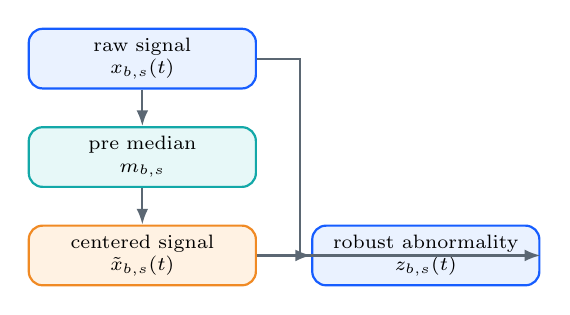
\begin{tikzpicture}[
  box/.style={rounded corners=5pt,draw=Blue,fill=SoftBlue,thick,text width=2.65cm,minimum height=0.75cm,align=center,font=\scriptsize},
  box2/.style={rounded corners=5pt,draw=Cyan,fill=SoftCyan,thick,text width=2.65cm,minimum height=0.75cm,align=center,font=\scriptsize},
  box3/.style={rounded corners=5pt,draw=Orange,fill=SoftOrange,thick,text width=2.65cm,minimum height=0.75cm,align=center,font=\scriptsize},
  arrow/.style={-{Latex[length=2mm]},thick,draw=Muted}
]
\node[box] (raw) at (0,1.6) {raw signal\\$x_{b,s}(t)$};
\node[box2] (med) at (0,0.35) {pre median\\$m_{b,s}$};
\node[box3] (center) at (0,-0.9) {centered signal\\$\tilde{x}_{b,s}(t)$};
\node[box] (z) at (3.6,-0.9) {robust abnormality\\$z_{b,s}(t)$};
\draw[arrow] (raw) -- (med);
\draw[arrow] (med) -- (center);
\draw[arrow] (center) -- (z);
\draw[arrow] (raw.east) -- ++(0.55,0) |- (z.east);
\end{tikzpicture}
\vspace{2mm}
\begin{alertblock}{Implementation detail}
If the MAD is too small, the code falls back to a standard deviation scale. If that also fails, it uses a safe fallback value.
\end{alertblock}
\end{column}
\end{columns}
\end{frame}

% -------------------------------------------------------------------
\begin{frame}{Baseline subtraction, visually}
\small
\begin{columns}[T,totalwidth=\textwidth]
\begin{column}{0.60\textwidth}
\centering
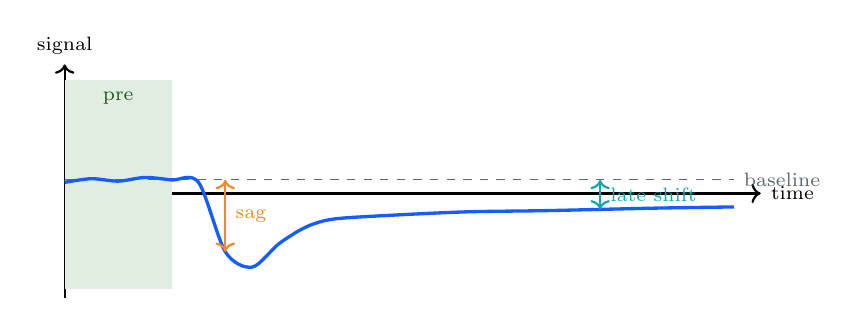
\begin{tikzpicture}[x=0.34cm,y=0.78cm]
  \draw[->,thick] (0,0) -- (26,0) node[right]{\scriptsize time};
  \draw[->,thick] (0,-1.7) -- (0,2.1) node[above]{\scriptsize signal};
  \fill[Green!14] (0,-1.55) rectangle (4,1.85);
  \node[Green!70!black] at (2,1.55) {\scriptsize pre};
  \draw[Muted,dashed] (0,0.22) -- (25,0.22) node[right]{\scriptsize baseline};
  \draw[Blue,very thick,smooth] plot coordinates {
    (0,0.18) (1,0.24) (2,0.20) (3,0.26) (4,0.22)
    (5,0.18) (6,-0.95) (7,-1.20) (8,-0.82) (9,-0.55)
    (10,-0.42) (12,-0.36) (15,-0.30) (18,-0.28) (22,-0.24) (25,-0.22)
  };
  \draw[Orange,<->,thick] (6,0.22) -- (6,-0.95) node[midway,right]{\scriptsize sag};
  \draw[Cyan,<->,thick] (20,0.22) -- (20,-0.26) node[midway,right]{\scriptsize late shift};
\end{tikzpicture}
\end{column}
\begin{column}{0.36\textwidth}
\begin{block}{What the model receives}
The feature extractor does not keep this curve. It records quantities such as early span, derivative, maximum deviation, and late shift.
\end{block}
\begin{exampleblock}{Fault reading}
A sharp voltage sag after the pre segment creates large derivative and large robust z-score features.
\end{exampleblock}
\end{column}
\end{columns}
\end{frame}

% -------------------------------------------------------------------
\begin{frame}{Feature naming convention}
\small
\begin{block}{Canonical pattern}
\[
\texttt{<PMU/BUS>\_\_<SIGNAL>\_\_<SEGMENT>\_\_<STATISTIC>}
\]
\end{block}
\begin{columns}[T,totalwidth=\textwidth]
\begin{column}{0.49\textwidth}
\begin{exampleblock}{Examples}
\code{Bus2\_\_VA\_MAG\_\_early\_\_span}\\
\code{Bus10\_\_Freq\_\_late\_\_mean}\\
\code{GLOBAL\_\_single\_signal\_score\_max}
\end{exampleblock}
\end{column}
\begin{column}{0.47\textwidth}
\begin{alertblock}{Reimplementation note}
The feature vector has tens of thousands of columns. A consistent naming scheme makes debugging and reimplementation possible.
\end{alertblock}
\end{column}
\end{columns}
\end{frame}

% -------------------------------------------------------------------
\section{Base Feature Engineering}

\begin{frame}[plain]{}
\begin{tikzpicture}[remember picture,overlay]
  \fill[Navy] (current page.south west) rectangle (current page.north east);
  \node[anchor=west] at ($(current page.west)+(0.8,0.6)$) {\color{Cyan}\Large Section 3};
  \node[anchor=west,text width=0.82\paperwidth] at ($(current page.west)+(0.8,-0.15)$) {\color{white}\Huge\bfseries Base Feature Engineering};
  \node[anchor=south east] at ($(current page.south east)+(-0.4,0.35)$) {\sgsmalogo[1.0cm]};
\end{tikzpicture}
\end{frame}

% -------------------------------------------------------------------
\begin{frame}{Base v2 feature families}
\small
\centering
\begin{tabular}{p{0.23\textwidth}p{0.34\textwidth}p{0.32\textwidth}}
\toprule
\textbf{Family} & \textbf{Computed from} & \textbf{Physical question}\\
\midrule
Segment statistics & every signal and segment & How large and variable was the response?\\
Temporal deltas & early/mid/late vs pre & Did the operating point move?\\
Derivatives & finite differences & How abrupt was the event?\\
Robust z-score & pre-event median/MAD & How abnormal was the signal?\\
Data quality & gaps, NaNs, data-present & Is this a measurement failure?\\
Single-signal anomaly & ranked abnormal channels & Is one channel corrupted?\\
Power proxy & V/I magnitudes and angles & Did active/reactive power change?\\
Global aggregations & PMU-level feature summaries & What is the system-wide pattern?\\
\bottomrule
\end{tabular}
\end{frame}

% -------------------------------------------------------------------
\begin{frame}{Feature factory: signal $\times$ segment $\times$ statistic}
\small
\centering
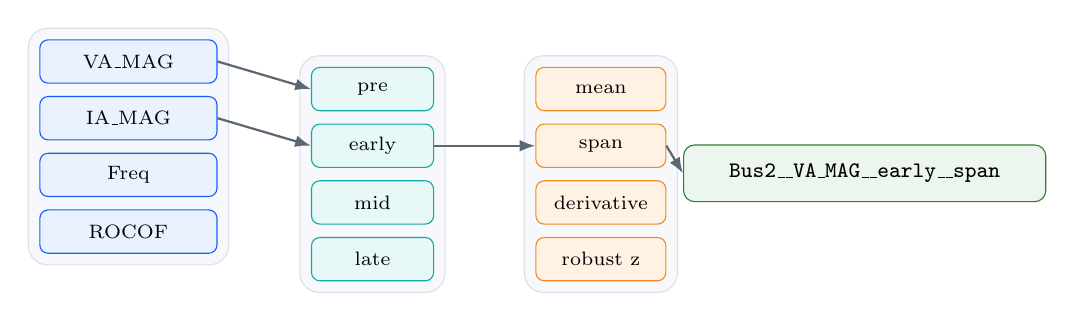
\begin{tikzpicture}[
  sig/.style={rounded corners=3pt,draw=Blue,fill=SoftBlue,minimum width=2.25cm,minimum height=0.55cm,font=\scriptsize},
  seg/.style={rounded corners=3pt,draw=Cyan,fill=SoftCyan,minimum width=1.55cm,minimum height=0.55cm,font=\scriptsize},
  stat/.style={rounded corners=3pt,draw=Orange,fill=SoftOrange,minimum width=1.65cm,minimum height=0.55cm,font=\scriptsize},
  outbox/.style={rounded corners=4pt,draw=Green,fill=SoftGreen,minimum width=4.6cm,minimum height=0.72cm,font=\scriptsize},
  arrow/.style={-{Latex[length=2mm]},thick,draw=Muted}
]
\node[sig] (s1) at (0,1.5) {VA\_MAG};
\node[sig] (s2) at (0,0.78) {IA\_MAG};
\node[sig] (s3) at (0,0.06) {Freq};
\node[sig] (s4) at (0,-0.66) {ROCOF};
\node[seg] (pre) at (3.1,1.15) {pre};
\node[seg] (early) at (3.1,0.43) {early};
\node[seg] (mid) at (3.1,-0.29) {mid};
\node[seg] (late) at (3.1,-1.01) {late};
\node[stat] (mean) at (6.0,1.15) {mean};
\node[stat] (span) at (6.0,0.43) {span};
\node[stat] (der) at (6.0,-0.29) {derivative};
\node[stat] (z) at (6.0,-1.01) {robust z};
\node[outbox] (out) at (9.35,0.08) {\code{Bus2\_\_VA\_MAG\_\_early\_\_span}};
\draw[arrow] (s1.east) -- (pre.west);
\draw[arrow] (s2.east) -- (early.west);
\draw[arrow] (early.east) -- (span.west);
\draw[arrow] (span.east) -- (out.west);
\begin{scope}[on background layer]
  \node[rounded corners=7pt,draw=Line,fill=Paper,fit=(s1)(s4),inner sep=4pt] {};
  \node[rounded corners=7pt,draw=Line,fill=Paper,fit=(pre)(late),inner sep=4pt] {};
  \node[rounded corners=7pt,draw=Line,fill=Paper,fit=(mean)(z),inner sep=4pt] {};
\end{scope}
\end{tikzpicture}
\vspace{3mm}
\begin{block}{Reimplementation shortcut}
Write the extractor as nested loops: for each PMU, for each signal, for each segment, compute the same statistics with the same names.
\end{block}
\end{frame}

% -------------------------------------------------------------------
\begin{frame}{Statistics generated inside each segment}
\small
\begin{columns}[T,totalwidth=\textwidth]
\begin{column}{0.49\textwidth}
\begin{block}{For centered values $\tilde{x}(t)$ in segment $\mathcal{S}$}
\[
\mu_{\mathcal{S}}=\frac{1}{|\mathcal{S}|}\sum_{t\in\mathcal{S}}\tilde{x}(t)
\]
\[
\sigma_{\mathcal{S}}=
\sqrt{\frac{1}{|\mathcal{S}|}\sum_{t\in\mathcal{S}}
\left(\tilde{x}(t)-\mu_{\mathcal{S}}\right)^2}
\]
\[
\mathrm{span}_{\mathcal{S}}=
\max_{t\in\mathcal{S}}\tilde{x}(t)-
\min_{t\in\mathcal{S}}\tilde{x}(t)
\]
\end{block}
\end{column}
\begin{column}{0.47\textwidth}
\begin{exampleblock}{Also stored}
\[
\min,\ \max,\ \mathrm{median},\ \max|\tilde{x}|,\ 
\mathrm{mean}|\tilde{x}|,\ p05,\ p95
\]
\end{exampleblock}
\centering
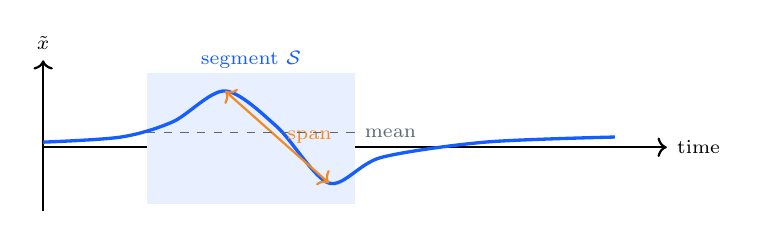
\begin{tikzpicture}[x=0.33cm,y=0.65cm]
  \draw[->,thick] (0,0) -- (24,0) node[right]{\scriptsize time};
  \draw[->,thick] (0,-1.25) -- (0,1.7) node[above]{\scriptsize $\tilde{x}$};
  \fill[Blue!10] (4,-1.1) rectangle (12,1.45);
  \node[Blue] at (8,1.7) {\scriptsize segment $\mathcal{S}$};
  \draw[Blue,very thick,smooth] plot coordinates {(0,0.1)(3,0.2)(5,0.5)(7,1.1)(9,0.4)(11,-0.7)(13,-0.2)(17,0.1)(22,0.2)};
  \draw[Orange,<->,thick] (11,-0.7) -- (7,1.1) node[midway,right]{\scriptsize span};
  \draw[Muted,dashed] (4,0.28) -- (12,0.28) node[right]{\scriptsize mean};
\end{tikzpicture}
\end{column}
\end{columns}
\end{frame}

% -------------------------------------------------------------------
\begin{frame}{Feature growth is controlled by loops}
\small
\centering
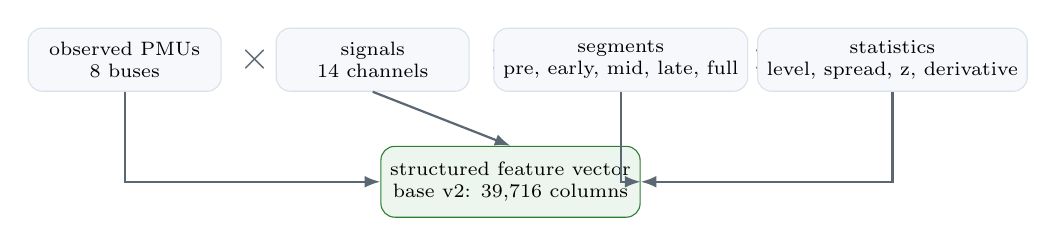
\begin{tikzpicture}[
  axis/.style={rounded corners=5pt,draw=Line,fill=Paper,minimum width=2.45cm,minimum height=0.8cm,align=center,font=\scriptsize},
  mult/.style={font=\Large\bfseries,color=Muted},
  outnode/.style={rounded corners=5pt,draw=Green,fill=SoftGreen,minimum width=3.1cm,minimum height=0.9cm,align=center,font=\scriptsize},
  arrow/.style={-{Latex[length=2mm]},thick,draw=Muted}
]
\node[axis] (bus) at (0,0) {observed PMUs\\8 buses};
\node[mult] at (1.65,0) {$\times$};
\node[axis] (sig) at (3.15,0) {signals\\14 channels};
\node[mult] at (4.8,0) {$\times$};
\node[axis] (seg) at (6.3,0) {segments\\pre, early, mid, late, full};
\node[mult] at (8.15,0) {$\times$};
\node[axis] (stat) at (9.75,0) {statistics\\level, spread, z, derivative};
\node[outnode] (feat) at (4.9,-1.55) {structured feature vector\\base v2: 39,716 columns};
\draw[arrow] (bus.south) |- (feat.west);
\draw[arrow] (sig.south) -- (feat.north);
\draw[arrow] (seg.south) |- (feat.east);
\draw[arrow] (stat.south) |- (feat.east);
\end{tikzpicture}
\vspace{4mm}
\begin{block}{Programming recipe}
Do not hand-write features. Generate names and values from loops, then freeze the resulting column order for training and inference.
\end{block}
\end{frame}

% -------------------------------------------------------------------
\begin{frame}{1. Segment statistics}
\small
\begin{block}{For each signal and each segment}
\[
\{\mathrm{mean},\ \mathrm{std},\ \mathrm{min},\ \mathrm{max},\ \mathrm{span},\ 
\mathrm{median},\ \mathrm{max\_abs},\ \mathrm{mean\_abs},\ p05,\ p95\}
\]
\end{block}
\begin{columns}[T,totalwidth=\textwidth]
\begin{column}{0.49\textwidth}
\begin{exampleblock}{Physical meaning}
\begin{itemize}
  \item \textbf{span}: event severity.
  \item \textbf{std}: oscillation or instability.
  \item \textbf{p05/p95}: stable extremes.
  \item \textbf{mean/median}: level shift.
\end{itemize}
\end{exampleblock}
\end{column}
\begin{column}{0.47\textwidth}
\begin{alertblock}{Event use}
Faults often create high voltage span; line outages produce current-span changes; generation/load events often produce sustained mean shifts.
\end{alertblock}
\end{column}
\end{columns}
\end{frame}

% -------------------------------------------------------------------
\begin{frame}{2. Temporal deltas}
\small
\begin{columns}[T,totalwidth=\textwidth]
\begin{column}{0.50\textwidth}
\begin{block}{Definitions}
\[
\Delta_{\mathrm{early}}=\mu_{\mathrm{early}}-\mu_{\mathrm{pre}}
\]
\[
\Delta_{\mathrm{mid}}=\mu_{\mathrm{mid}}-\mu_{\mathrm{pre}}
\]
\[
\Delta_{\mathrm{late}}=\mu_{\mathrm{late}}-\mu_{\mathrm{pre}}
\]
\end{block}
\end{column}
\begin{column}{0.46\textwidth}
\begin{exampleblock}{Interpretation}
\begin{itemize}
  \item early delta: onset shock.
  \item mid delta: transient settling.
  \item late delta: persistent operating-point change.
\end{itemize}
\end{exampleblock}
\end{column}
\end{columns}
\vspace{2mm}
\begin{alertblock}{Why not only full-window stats?}
Two windows can have the same full-window mean but different temporal behavior. The deltas preserve event timing.
\end{alertblock}
\end{frame}

% -------------------------------------------------------------------
\begin{frame}{3. Derivative features}
\small
\begin{block}{Finite-difference approximation}
\[
d_x(t) = \frac{x(t)-x(t-\Delta t)}{\Delta t}
\]
\[
\mathrm{max\_abs\_derivative}=\max_t |d_x(t)|,\qquad
\mathrm{rms\_derivative}=\sqrt{\frac{1}{T}\sum_t d_x(t)^2}
\]
\end{block}
\begin{columns}[T,totalwidth=\textwidth]
\begin{column}{0.47\textwidth}
\begin{exampleblock}{High derivative}
Usually means an abrupt transient: fault onset, line switching, or corrupted data.
\end{exampleblock}
\end{column}
\begin{column}{0.49\textwidth}
\begin{alertblock}{Event use}
The final rule engine uses voltage and current derivative thresholds to guard fault and line-outage decisions.
\end{alertblock}
\end{column}
\end{columns}
\end{frame}

% -------------------------------------------------------------------
\begin{frame}{4. Robust z-score}
\small
\begin{block}{Robust scale from the pre-event segment}
\[
m=\mathrm{median}(x_{\mathrm{pre}}),\qquad
\mathrm{MAD}=\mathrm{median}(|x_{\mathrm{pre}}-m|)
\]
\[
z_{\mathrm{robust}}(t)=\frac{|x(t)-m|}{\mathrm{MAD}+\epsilon}
\]
\end{block}
\begin{columns}[T,totalwidth=\textwidth]
\begin{column}{0.47\textwidth}
\begin{exampleblock}{Features}
\begin{itemize}
  \item \code{max\_abs\_robust\_z}
  \item \code{sustained\_abs\_robust\_z\_5}
  \item \code{sustained\_abs\_robust\_z\_15}
\end{itemize}
\end{exampleblock}
\end{column}
\begin{column}{0.49\textwidth}
\begin{alertblock}{Why median/MAD here}
The median and MAD are less sensitive to spikes than mean and standard deviation, which matters when bad data is one of the event classes.
\end{alertblock}
\end{column}
\end{columns}
\end{frame}

% -------------------------------------------------------------------
\begin{frame}{Robust z-score separates two failure modes}
\small
\begin{columns}[T,totalwidth=\textwidth]
\begin{column}{0.50\textwidth}
\centering
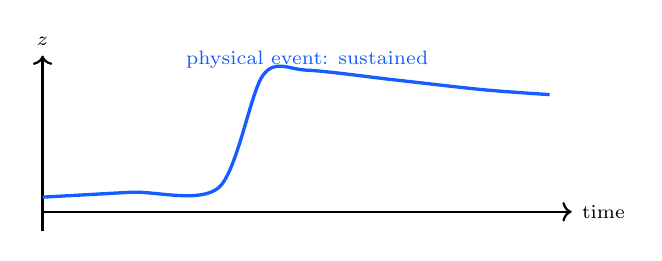
\begin{tikzpicture}[x=0.28cm,y=0.62cm]
  \draw[->,thick] (0,0) -- (24,0) node[right]{\scriptsize time};
  \draw[->,thick] (0,-0.4) -- (0,3.2) node[above]{\scriptsize $z$};
  \draw[Blue,very thick,smooth] plot coordinates {(0,0.3)(4,0.4)(8,0.5)(10,2.8)(12,2.9)(16,2.7)(20,2.5)(23,2.4)};
  \node[Blue] at (12,3.12) {\scriptsize physical event: sustained};
\end{tikzpicture}\\[1mm]
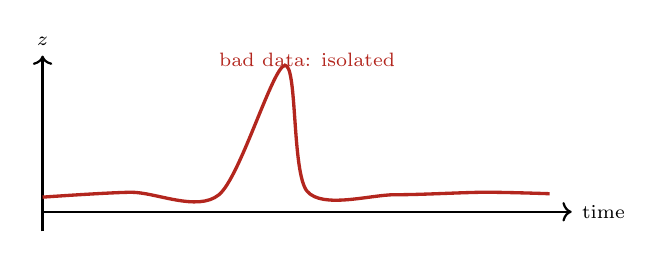
\begin{tikzpicture}[x=0.28cm,y=0.62cm]
  \draw[->,thick] (0,0) -- (24,0) node[right]{\scriptsize time};
  \draw[->,thick] (0,-0.4) -- (0,3.2) node[above]{\scriptsize $z$};
  \draw[Red,very thick,smooth] plot coordinates {(0,0.3)(4,0.4)(8,0.35)(11,3.0)(12,0.42)(16,0.35)(20,0.40)(23,0.37)};
  \node[Red] at (12,3.12) {\scriptsize bad data: isolated};
\end{tikzpicture}
\end{column}
\begin{column}{0.46\textwidth}
\begin{block}{Why we keep both max and sustained scores}
\code{max\_abs\_robust\_z} catches the spike. Sustained features say whether the abnormal value stays high for several samples.
\end{block}
\begin{alertblock}{Classifier use}
The pair helps the event model avoid calling every spike a physical event.
\end{alertblock}
\end{column}
\end{columns}
\end{frame}

% -------------------------------------------------------------------
\begin{frame}{5. Sustained anomaly features}
\small
\begin{block}{Concept}
Not every high z-score is equally meaningful. A single spike may be bad data; a sustained high z-score may be a physical event.
\end{block}
\begin{columns}[T,totalwidth=\textwidth]
\begin{column}{0.48\textwidth}
\begin{exampleblock}{Short sustained score}
\code{sustained\_abs\_robust\_z\_5}\\
Captures short bursts and sharp events.
\end{exampleblock}
\end{column}
\begin{column}{0.48\textwidth}
\begin{exampleblock}{Long sustained score}
\code{sustained\_abs\_robust\_z\_15}\\
Captures persistent deviations after the event.
\end{exampleblock}
\end{column}
\end{columns}
\vspace{2mm}
\begin{alertblock}{Practical reading}
Faults can be sharp and sustained; bad data is often isolated to one channel; load/generation changes persist in late features.
\end{alertblock}
\end{frame}

% -------------------------------------------------------------------
\begin{frame}{6. Data-quality features}
\small
\begin{columns}[T,totalwidth=\textwidth]
\begin{column}{0.53\textwidth}
\begin{block}{Features}
\begin{itemize}
  \item \code{n\_samples}, \code{duration\_s}, \code{dt\_s}
  \item \code{max\_timestamp\_gap\_s}
  \item \code{max\_timestamp\_gap\_ratio}
  \item \code{data\_present\_fraction}
  \item \code{data\_present\_min}
  \item \code{missing\_run\_max\_samples}
  \item \code{missing\_run\_max\_s}
  \item \code{nan\_fraction\_max/mean}
\end{itemize}
\end{block}
\end{column}
\begin{column}{0.43\textwidth}
\begin{alertblock}{Decision logic}
\[
\mathrm{missing} \Rightarrow
\begin{cases}
\mathrm{Event\ 5}, & \text{no physical event}\\
\mathrm{Event\ 6}, & \text{physical event also present}
\end{cases}
\]
\end{alertblock}
\begin{exampleblock}{Physical meaning}
Missing-data events are communication or measurement failures, not necessarily grid disturbances.
\end{exampleblock}
\end{column}
\end{columns}
\end{frame}

% -------------------------------------------------------------------
\begin{frame}{7. Single-signal bad-data features}
\small
\begin{block}{Goal}
Detect a channel that becomes extreme while the rest of the PMU/grid remains coherent.
\end{block}
\begin{columns}[T,totalwidth=\textwidth]
\begin{column}{0.50\textwidth}
\begin{exampleblock}{Features}
\begin{itemize}
  \item \code{single\_signal\_score\_max}
  \item \code{single\_signal\_score\_second}
  \item \code{single\_signal\_score\_ratio}
  \item \code{single\_signal\_score\_count\_gt20}
\end{itemize}
\end{exampleblock}
\end{column}
\begin{column}{0.46\textwidth}
\begin{alertblock}{Rule of thumb}
\[
\frac{\mathrm{top\ anomaly}}{\mathrm{second\ anomaly}} \ge 3
\Rightarrow \mathrm{bad\ data\ candidate}
\]
\end{alertblock}
\end{column}
\end{columns}
\end{frame}

% -------------------------------------------------------------------
\begin{frame}{8. Phase-spread and consistency features}
\small
\begin{block}{What is measured}
For voltage/current magnitude and angle groups, the extractor summarizes phase-to-phase spread and consistency.
\end{block}
\begin{columns}[T,totalwidth=\textwidth]
\begin{column}{0.48\textwidth}
\begin{exampleblock}{Physical role}
\begin{itemize}
  \item three-phase imbalance,
  \item phase-angle inconsistency,
  \item PMU channel mismatch.
\end{itemize}
\end{exampleblock}
\end{column}
\begin{column}{0.48\textwidth}
\begin{alertblock}{Event use}
These features help separate grid events from measurement artifacts because real events tend to preserve more cross-phase structure than corrupted channels.
\end{alertblock}
\end{column}
\end{columns}
\end{frame}

% -------------------------------------------------------------------
\begin{frame}{Power proxy from voltage-current phase angle}
\small
\begin{columns}[T,totalwidth=\textwidth]
\begin{column}{0.47\textwidth}
\begin{block}{Per-unit magnitudes}
\[
V_{pu,\phi}(t)=
\frac{|V_{\phi}(t)|}
{\max(\mathrm{median}_{pre}|V_{\phi}|,\epsilon)}
\]
\[
I_{pu,\phi}(t)=
\frac{|I_{\phi}(t)|}
{\max(\mathrm{median}_{pre}|I_{\phi}|,\epsilon)}
\]
\end{block}
\begin{alertblock}{Proxy, not calibrated power}
The challenge data does not require a full power-flow solve. The proxy gives the classifier a stable signature of active/reactive behavior.
\end{alertblock}
\end{column}
\begin{column}{0.49\textwidth}
\centering
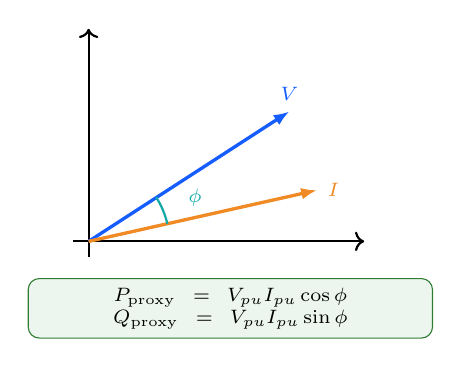
\begin{tikzpicture}[scale=1.0]
  \draw[->,thick] (-0.2,0) -- (3.5,0);
  \draw[->,thick] (0,-0.2) -- (0,2.7);
  \draw[Blue,very thick,-{Latex[length=2mm]}] (0,0) -- (2.55,1.65) node[above]{\scriptsize $V$};
  \draw[Orange,very thick,-{Latex[length=2mm]}] (0,0) -- (2.9,0.65) node[right]{\scriptsize $I$};
  \draw[Cyan,thick] (1.0,0.22) arc[start angle=12.6,end angle=32.9,radius=1.05];
  \node[Cyan] at (1.35,0.55) {\scriptsize $\phi$};
  \node[rounded corners=4pt,draw=Green,fill=SoftGreen,text width=4.9cm,align=center,font=\scriptsize] at (1.8,-0.85)
  {$P_{\mathrm{proxy}}=V_{pu}I_{pu}\cos\phi$\\$Q_{\mathrm{proxy}}=V_{pu}I_{pu}\sin\phi$};
\end{tikzpicture}
\vspace{1mm}
\begin{exampleblock}{Electrical reading}
A load or generation change can shift $I$, $\phi$, and frequency while voltage magnitude remains moderate.
\end{exampleblock}
\end{column}
\end{columns}
\end{frame}

% -------------------------------------------------------------------
\begin{frame}{9. Power proxy features}
\small
\begin{columns}[T,totalwidth=\textwidth]
\begin{column}{0.52\textwidth}
\begin{block}{Per phase}
\[
\phi = \theta_V - \theta_I
\]
\[
P_{\mathrm{proxy}} = V_{\mathrm{pu}} I_{\mathrm{pu}} \cos(\phi)
\]
\[
Q_{\mathrm{proxy}} = V_{\mathrm{pu}} I_{\mathrm{pu}} \sin(\phi)
\]
\[
PF_{\mathrm{ang}} = \phi
\]
\end{block}
\end{column}
\begin{column}{0.44\textwidth}
\begin{exampleblock}{Use in classifier}
Generation and load events may not create dramatic voltage disturbances. They are often easier to see through frequency, current, and active/reactive power proxy changes.
\end{exampleblock}
\begin{alertblock}{Used most by}
Event 3, Event 4, and mixed physical Event 8.
\end{alertblock}
\end{column}
\end{columns}
\end{frame}

% -------------------------------------------------------------------
\begin{frame}{10. Global PMU aggregation}
\small
\begin{block}{What is aggregated}
After extracting bus-level features, the model also computes global summaries across observed PMUs:
\[
\mathrm{mean},\ \mathrm{max},\ \mathrm{min},\ \mathrm{std}
\]
\end{block}
\begin{exampleblock}{Why it helps}
A local event has a spatial footprint. Global aggregation gives the classifier a system-level view: is the disturbance concentrated, widespread, coherent, or isolated?
\end{exampleblock}
\begin{alertblock}{Example}
Bad data often has one extreme PMU/channel. A physical event affects multiple PMUs in a structured way.
\end{alertblock}
\end{frame}

% -------------------------------------------------------------------
\begin{frame}{Base feature count}
\small
\centering
\begin{tabular}{lr}
\toprule
\textbf{Feature group} & \textbf{Count}\\
\midrule
Voltage angle & 7,596\\
Voltage magnitude & 7,596\\
Current angle & 7,596\\
Current magnitude & 7,596\\
Frequency / ROCOF & 4,640\\
Power proxy & 4,428\\
Data quality & 156\\
Single-signal anomaly & 48\\
Other/global & 60\\
\midrule
\textbf{Base v2 total} & \textbf{39,716}\\
\bottomrule
\end{tabular}
\vspace{3mm}
\begin{block}{Reimplementation note}
The base model uses a large but structured feature vector. The structure is what makes it reimplementable.
\end{block}
\end{frame}

% -------------------------------------------------------------------
\section{Dynamic Feature Engineering}

\begin{frame}[plain]{}
\begin{tikzpicture}[remember picture,overlay]
  \fill[Navy] (current page.south west) rectangle (current page.north east);
  \node[anchor=west] at ($(current page.west)+(0.8,0.6)$) {\color{Cyan}\Large Section 4};
  \node[anchor=west,text width=0.82\paperwidth] at ($(current page.west)+(0.8,-0.15)$) {\color{white}\Huge\bfseries Dynamic Feature Engineering};
  \node[anchor=south east] at ($(current page.south east)+(-0.4,0.35)$) {\sgsmalogo[1.0cm]};
\end{tikzpicture}
\end{frame}

% -------------------------------------------------------------------
\begin{frame}{Why dynamic features were added}
\small
\begin{block}{Base features answer}
How large, abnormal, and persistent was the signal within each segment?
\end{block}
\begin{alertblock}{Dynamic features answer}
How did the signal evolve across time scales, and how did the disturbance propagate across PMUs?
\end{alertblock}
\begin{columns}[T,totalwidth=\textwidth]
\begin{column}{0.32\textwidth}
\begin{exampleblock}{Rolling}
Multi-scale local behavior.
\end{exampleblock}
\end{column}
\begin{column}{0.32\textwidth}
\begin{exampleblock}{RLS/Kalman}
Prediction residuals and innovations.
\end{exampleblock}
\end{column}
\begin{column}{0.32\textwidth}
\begin{exampleblock}{Graph temporal}
Spatial-temporal PMU signature.
\end{exampleblock}
\end{column}
\end{columns}
\end{frame}

% -------------------------------------------------------------------
\begin{frame}{Dynamic blocks as engineering questions}
\small
\centering
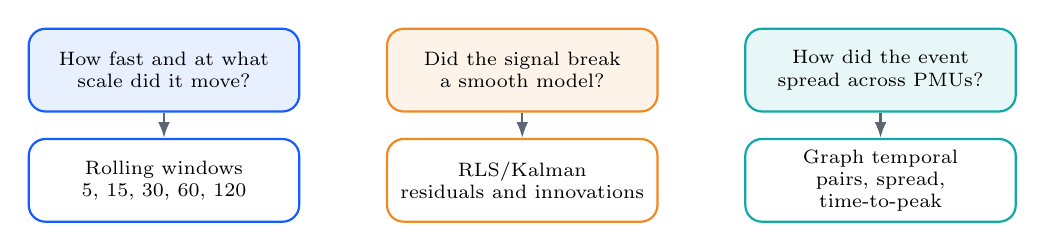
\begin{tikzpicture}[
  qblue/.style={rounded corners=6pt,draw=Blue,fill=Blue!10,thick,text width=3.2cm,minimum height=1.05cm,align=center,font=\scriptsize},
  ablue/.style={rounded corners=6pt,draw=Blue,fill=white,thick,text width=3.2cm,minimum height=1.05cm,align=center,font=\scriptsize},
  qorange/.style={rounded corners=6pt,draw=Orange,fill=Orange!10,thick,text width=3.2cm,minimum height=1.05cm,align=center,font=\scriptsize},
  aorange/.style={rounded corners=6pt,draw=Orange,fill=white,thick,text width=3.2cm,minimum height=1.05cm,align=center,font=\scriptsize},
  qcyan/.style={rounded corners=6pt,draw=Cyan,fill=Cyan!10,thick,text width=3.2cm,minimum height=1.05cm,align=center,font=\scriptsize},
  acyan/.style={rounded corners=6pt,draw=Cyan,fill=white,thick,text width=3.2cm,minimum height=1.05cm,align=center,font=\scriptsize},
  arrow/.style={-{Latex[length=2mm]},thick,draw=Muted}
]
\node[qblue] (q1) at (0,1.4) {How fast and at what scale did it move?};
\node[ablue] (a1) at (0,0) {Rolling windows\\5, 15, 30, 60, 120};
\node[qorange] (q2) at (4.55,1.4) {Did the signal break a smooth model?};
\node[aorange] (a2) at (4.55,0) {RLS/Kalman\\residuals and innovations};
\node[qcyan] (q3) at (9.1,1.4) {How did the event spread across PMUs?};
\node[acyan] (a3) at (9.1,0) {Graph temporal\\pairs, spread, time-to-peak};
\draw[arrow] (q1) -- (a1);
\draw[arrow] (q2) -- (a2);
\draw[arrow] (q3) -- (a3);
\end{tikzpicture}
\vspace{3mm}
\begin{block}{Implementation reading}
Each dynamic block is a small, testable module. You can add them one at a time after the base extractor works.
\end{block}
\end{frame}

% -------------------------------------------------------------------
\begin{frame}{Signals used in dynamic extraction}
\small
\begin{block}{Main signal set}
\[
\{\mathrm{VA/VB/VC\_MAG},\ \mathrm{IA/IB/IC\_MAG},\ \mathrm{VA/VB/VC\_ANG},\ \mathrm{IA/IB/IC\_ANG},\ \mathrm{Freq},\ \mathrm{ROCOF}\}
\]
\end{block}
\begin{exampleblock}{Reduced signal set for RLS/Kalman and graph features}
\[
\{\mathrm{VA\_MAG},\ \mathrm{IA\_MAG},\ \mathrm{VA\_ANG},\ \mathrm{IA\_ANG},\ \mathrm{Freq},\ \mathrm{ROCOF}\}
\]
\end{exampleblock}
\begin{alertblock}{Reason}
The reduced set keeps dynamic features feasible while preserving representative voltage, current, angle, and frequency behavior.
\end{alertblock}
\end{frame}

% -------------------------------------------------------------------
\begin{frame}{Dynamic extractor: same signal, three views}
\small
\centering
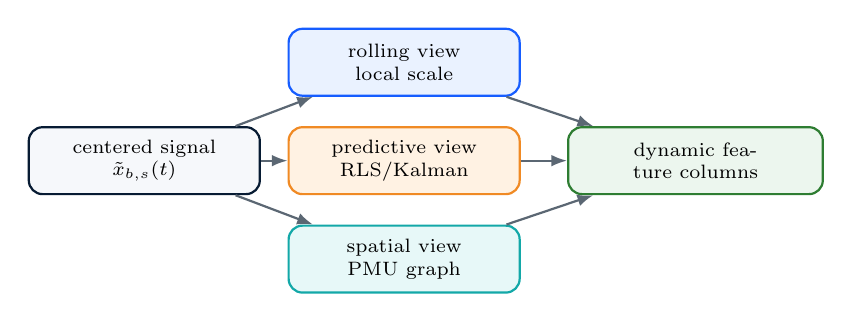
\begin{tikzpicture}[
  node distance=0.75cm,
  raw/.style={rounded corners=5pt,draw=Navy,fill=Paper,thick,text width=2.7cm,minimum height=0.85cm,align=center,font=\scriptsize},
  roll/.style={rounded corners=5pt,draw=Blue,fill=SoftBlue,thick,text width=2.7cm,minimum height=0.85cm,align=center,font=\scriptsize},
  rls/.style={rounded corners=5pt,draw=Orange,fill=SoftOrange,thick,text width=2.7cm,minimum height=0.85cm,align=center,font=\scriptsize},
  graph/.style={rounded corners=5pt,draw=Cyan,fill=SoftCyan,thick,text width=2.7cm,minimum height=0.85cm,align=center,font=\scriptsize},
  outbox/.style={rounded corners=5pt,draw=Green,fill=SoftGreen,thick,text width=3.0cm,minimum height=0.85cm,align=center,font=\scriptsize},
  arrow/.style={-{Latex[length=2mm]},thick,draw=Muted}
]
\node[raw] (x) at (0,0) {centered signal\\$\tilde{x}_{b,s}(t)$};
\node[roll] (r) at (3.3,1.25) {rolling view\\local scale};
\node[rls] (k) at (3.3,0) {predictive view\\RLS/Kalman};
\node[graph] (g) at (3.3,-1.25) {spatial view\\PMU graph};
\node[outbox] (f) at (7.0,0) {dynamic feature columns};
\draw[arrow] (x) -- (r);
\draw[arrow] (x) -- (k);
\draw[arrow] (x) -- (g);
\draw[arrow] (r) -- (f);
\draw[arrow] (k) -- (f);
\draw[arrow] (g) -- (f);
\end{tikzpicture}
\vspace{3mm}
\begin{block}{Implementation reading}
All dynamic blocks start after baseline subtraction. That makes the blocks comparable across buses and across RAW/SIM cases.
\end{block}
\end{frame}

% -------------------------------------------------------------------
\begin{frame}{Rolling multi-scale features}
\small
\begin{columns}[T,totalwidth=\textwidth]
\begin{column}{0.45\textwidth}
\begin{block}{Rolling windows}
\[
w \in \{5,15,30,60,120\}
\]
\end{block}
\begin{block}{Features}
\begin{itemize}
  \item \code{mean\_abs\_max}
  \item \code{std\_max}, \code{std\_mean}
  \item \code{slope\_max\_abs}
  \item \code{energy}
  \item \code{time\_to\_abs\_peak}
\end{itemize}
\end{block}
\end{column}
\begin{column}{0.51\textwidth}
\begin{exampleblock}{Physical interpretation}
\begin{itemize}
  \item short windows catch abrupt switching/fault onset;
  \item long windows catch sustained load/generation shifts;
  \item time-to-peak helps localize event propagation.
\end{itemize}
\end{exampleblock}
\end{column}
\end{columns}
\end{frame}

% -------------------------------------------------------------------
\begin{frame}{Rolling block equations and plot}
\small
\begin{columns}[T,totalwidth=\textwidth]
\begin{column}{0.49\textwidth}
\begin{block}{Centered rolling mean and standard deviation}
\[
\mu_w(t)=\frac{1}{w}\sum_{\tau\in W_w(t)}\tilde{x}(\tau)
\]
\[
\sigma_w(t)=
\sqrt{\frac{1}{w}\sum_{\tau\in W_w(t)}
\left(\tilde{x}(\tau)-\mu_w(t)\right)^2}
\]
\[
E_x=\frac{1}{T}\sum_t|\tilde{x}(t)|^2
\]
\end{block}
\end{column}
\begin{column}{0.47\textwidth}
\centering
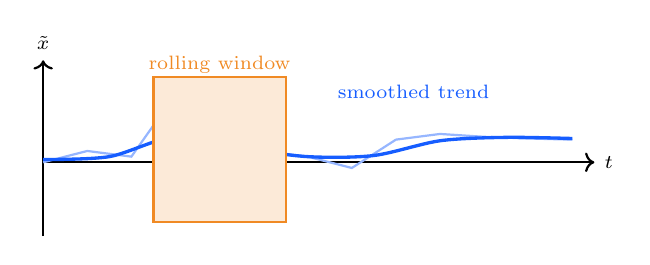
\begin{tikzpicture}[x=0.28cm,y=0.72cm]
  \draw[->,thick] (0,0) -- (25,0) node[right]{\scriptsize $t$};
  \draw[->,thick] (0,-1.3) -- (0,1.8) node[above]{\scriptsize $\tilde{x}$};
  \draw[Blue!45,thick] plot coordinates {(0,0.0)(2,0.2)(4,0.1)(6,1.2)(8,-0.6)(10,0.2)(12,0.1)(14,-0.1)(16,0.4)(18,0.5)(20,0.45)(22,0.42)(24,0.40)};
  \draw[Blue,very thick,smooth] plot coordinates {(0,0.05)(3,0.1)(6,0.45)(9,0.25)(12,0.1)(15,0.12)(18,0.38)(21,0.44)(24,0.42)};
  \fill[Orange!18] (5,-1.05) rectangle (11,1.5);
  \draw[Orange,thick] (5,-1.05) rectangle (11,1.5);
  \node[Orange] at (8,1.72) {\scriptsize rolling window};
  \node[Blue] at (16.8,1.25) {\scriptsize smoothed trend};
\end{tikzpicture}
\vspace{2mm}
\begin{exampleblock}{Stored for each $w$}
\[
\max|\mu_w|,\quad \max\sigma_w,\quad \overline{\sigma_w},\quad
\max\left|\frac{d\mu_w}{dt}\right|,\quad E_x,\quad t_{\mathrm{peak}}
\]
\end{exampleblock}
\end{column}
\end{columns}
\end{frame}

% -------------------------------------------------------------------
\begin{frame}{RLS/Kalman residual features}
\small
\begin{block}{Concept}
Fit a simple expected trajectory. If the actual signal deviates sharply from that expected trajectory, the residual or innovation becomes large.
\end{block}
\begin{columns}[T,totalwidth=\textwidth]
\begin{column}{0.49\textwidth}
\begin{exampleblock}{RLS-style features}
\begin{itemize}
  \item \code{level\_resid}
  \item \code{theta\_delta}
  \item \code{linear\_resid}
  \item forgetting factors: 0.92 and 0.985
\end{itemize}
\end{exampleblock}
\end{column}
\begin{column}{0.47\textwidth}
\begin{alertblock}{Kalman-style features}
\begin{itemize}
  \item \code{kalman\_innov}
  \item max, mean, p95
  \item time-to-peak
\end{itemize}
\end{alertblock}
\end{column}
\end{columns}
\end{frame}

% -------------------------------------------------------------------
\begin{frame}{RLS constant-level model}
\small
\begin{columns}[T,totalwidth=\textwidth]
\begin{column}{0.52\textwidth}
\begin{block}{Model}
\[
y_t=\theta_t+e_t
\]
\[
K_t=\frac{P_{t-1}}{\lambda+P_{t-1}}
\]
\[
\theta_t=\theta_{t-1}+K_t(y_t-\theta_{t-1})
\]
\[
P_t=\frac{P_{t-1}-K_tP_{t-1}}{\lambda}
\]
\end{block}
\begin{exampleblock}{Forgetting factors}
\[
\lambda\in\{0.92,\ 0.985\}
\]
\end{exampleblock}
\end{column}
\begin{column}{0.44\textwidth}
\begin{alertblock}{Features produced}
\[
r_t=|y_t-\theta_{t-1}|
\]
\[
\Delta\theta_t=|\theta_t-\theta_{t-1}|
\]
For each sequence:
\[
\max,\quad \mathrm{mean},\quad p95,\quad
\mathrm{median}_{late}-\mathrm{median}_{pre}
\]
\end{alertblock}
\centering
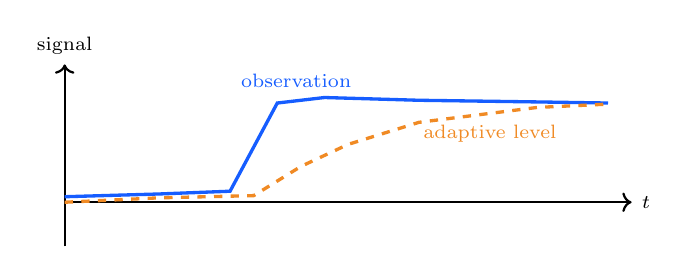
\begin{tikzpicture}[x=0.30cm,y=0.70cm]
  \draw[->,thick] (0,0) -- (24,0) node[right]{\scriptsize $t$};
  \draw[->,thick] (0,-0.8) -- (0,2.5) node[above]{\scriptsize signal};
  \draw[Blue,very thick] plot coordinates {(0,0.1)(4,0.15)(7,0.2)(9,1.8)(11,1.9)(15,1.85)(20,1.82)(23,1.8)};
  \draw[Orange,very thick,dashed] plot coordinates {(0,0.0)(4,0.08)(8,0.12)(10,0.65)(12,1.05)(15,1.45)(20,1.72)(23,1.78)};
  \node[Blue] at (9.8,2.2) {\scriptsize observation};
  \node[Orange] at (18,1.25) {\scriptsize adaptive level};
\end{tikzpicture}
\end{column}
\end{columns}
\end{frame}

% -------------------------------------------------------------------
\begin{frame}{RLS linear-trend model}
\small
\begin{columns}[T,totalwidth=\textwidth]
\begin{column}{0.53\textwidth}
\begin{block}{Local linear predictor}
\[
\phi_t=\begin{bmatrix}1\\t-t_0\end{bmatrix},
\qquad
\hat{y}_t=\phi_t^\top\theta_{t-1}
\]
\[
K_t=\frac{P_{t-1}\phi_t}
{\lambda+\phi_t^\top P_{t-1}\phi_t}
\]
\[
\theta_t=\theta_{t-1}+K_t(y_t-\hat{y}_t)
\]
\[
P_t=\frac{P_{t-1}-K_t\phi_t^\top P_{t-1}}{\lambda}
\]
\end{block}
\end{column}
\begin{column}{0.43\textwidth}
\centering
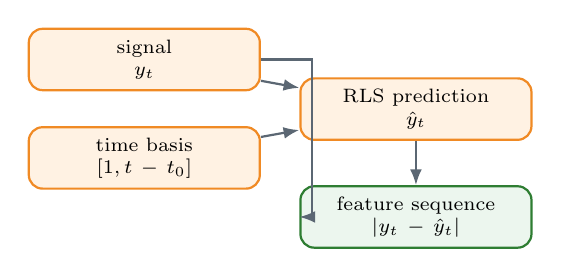
\begin{tikzpicture}[
  box/.style={rounded corners=5pt,draw=Orange,fill=SoftOrange,thick,text width=2.7cm,minimum height=0.78cm,align=center,font=\scriptsize},
  outbox/.style={rounded corners=5pt,draw=Green,fill=SoftGreen,thick,text width=2.7cm,minimum height=0.78cm,align=center,font=\scriptsize},
  arrow/.style={-{Latex[length=2mm]},thick,draw=Muted}
]
\node[box] (x) at (0,1.35) {signal\\$y_t$};
\node[box] (phi) at (0,0.1) {time basis\\$[1,t-t_0]$};
\node[box] (pred) at (3.45,0.72) {RLS prediction\\$\hat{y}_t$};
\node[outbox] (res) at (3.45,-0.65) {feature sequence\\$|y_t-\hat{y}_t|$};
\draw[arrow] (x) -- (pred);
\draw[arrow] (phi) -- (pred);
\draw[arrow] (pred) -- (res);
\draw[arrow] (x.east) -- ++(0.65,0) |- (res.west);
\end{tikzpicture}
\vspace{3mm}
\begin{exampleblock}{Why linear residuals help}
They discount smooth ramps but react to switching, faults, and sudden sensor errors.
\end{exampleblock}
\end{column}
\end{columns}
\end{frame}

% -------------------------------------------------------------------
\begin{frame}{Kalman level model used in the dynamic block}
\small
\begin{columns}[T,totalwidth=\textwidth]
\begin{column}{0.52\textwidth}
\begin{block}{State-space view}
\[
x_t=x_{t-1}+w_t,\qquad w_t\sim\mathcal{N}(0,Q)
\]
\[
y_t=x_t+v_t,\qquad v_t\sim\mathcal{N}(0,R)
\]
\[
Q=(0.005\,s)^2,\qquad R=(0.08\,s)^2
\]
\[
s=\mathrm{robust\_scale}(y)
\]
\end{block}
\end{column}
\begin{column}{0.44\textwidth}
\begin{alertblock}{Update equations}
\[
P_t^- = P_{t-1}+Q
\]
\[
\nu_t=y_t-\hat{x}_{t-1}
\]
\[
K_t=\frac{P_t^-}{P_t^-+R}
\]
\[
\hat{x}_t=\hat{x}_{t-1}+K_t\nu_t,\qquad
P_t=(1-K_t)P_t^-
\]
\end{alertblock}
\end{column}
\end{columns}
\vspace{1mm}
\begin{exampleblock}{Feature sequence}
The stored signal is $|\nu_t|$, the absolute innovation. A large innovation means the measurement did not match the smooth level model.
\end{exampleblock}
\end{frame}

% -------------------------------------------------------------------
\begin{frame}{Kalman innovation diagram}
\small
\begin{columns}[T,totalwidth=\textwidth]
\begin{column}{0.57\textwidth}
\centering
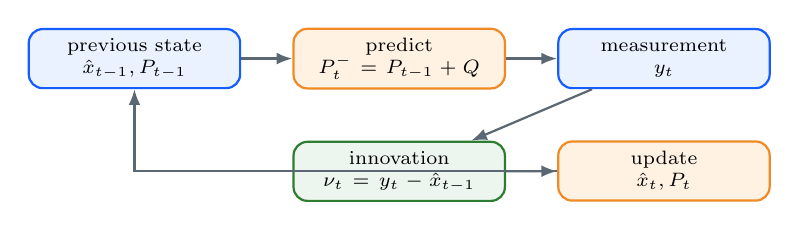
\begin{tikzpicture}[
  node distance=0.65cm,
  box/.style={rounded corners=5pt,draw=Blue,fill=SoftBlue,thick,text width=2.45cm,minimum height=0.75cm,align=center,font=\scriptsize},
  box2/.style={rounded corners=5pt,draw=Orange,fill=SoftOrange,thick,text width=2.45cm,minimum height=0.75cm,align=center,font=\scriptsize},
  box3/.style={rounded corners=5pt,draw=Green,fill=SoftGreen,thick,text width=2.45cm,minimum height=0.75cm,align=center,font=\scriptsize},
  arrow/.style={-{Latex[length=2mm]},thick,draw=Muted}
]
\node[box] (prev) at (0,0) {previous state\\$\hat{x}_{t-1},P_{t-1}$};
\node[box2,right=of prev] (pred) {predict\\$P^-_t=P_{t-1}+Q$};
\node[box,right=of pred] (meas) {measurement\\$y_t$};
\node[box3,below=of pred] (innov) {innovation\\$\nu_t=y_t-\hat{x}_{t-1}$};
\node[box2,below=of meas] (upd) {update\\$\hat{x}_t,P_t$};
\draw[arrow] (prev) -- (pred);
\draw[arrow] (pred) -- (meas);
\draw[arrow] (meas) -- (innov);
\draw[arrow] (innov) -- (upd);
\draw[arrow] (upd.west) -| (prev.south);
\end{tikzpicture}
\end{column}
\begin{column}{0.39\textwidth}
\centering
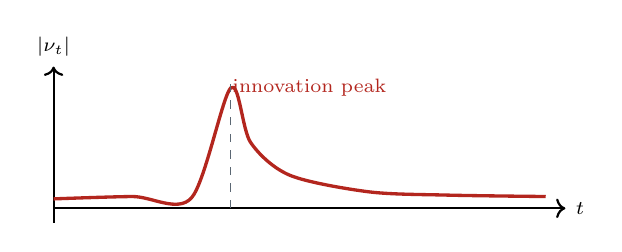
\begin{tikzpicture}[x=0.25cm,y=0.60cm]
  \draw[->,thick] (0,0) -- (26,0) node[right]{\scriptsize $t$};
  \draw[->,thick] (0,-0.3) -- (0,3.0) node[above]{\scriptsize $|\nu_t|$};
  \draw[Red,very thick,smooth] plot coordinates {(0,0.2)(4,0.25)(7,0.22)(9,2.55)(10,1.4)(12,0.7)(16,0.35)(20,0.28)(25,0.25)};
  \draw[Muted,dashed] (9,0) -- (9,2.65);
  \node[Red] at (13,2.55) {\scriptsize innovation peak};
\end{tikzpicture}
\vspace{2mm}
\begin{exampleblock}{Stored features}
\[
\max|\nu_t|,\quad \mathrm{mean}|\nu_t|,\quad p95|\nu_t|,\quad
t_{\mathrm{peak}}
\]
\end{exampleblock}
\end{column}
\end{columns}
\end{frame}

% -------------------------------------------------------------------
\begin{frame}{How RLS/Kalman separates event shapes}
\small
\begin{columns}[T,totalwidth=\textwidth]
\begin{column}{0.50\textwidth}
\centering
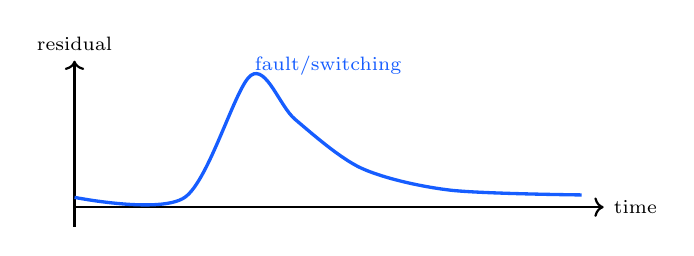
\begin{tikzpicture}[x=0.28cm,y=0.62cm]
  \draw[->,thick] (0,0) -- (24,0) node[right]{\scriptsize time};
  \draw[->,thick] (0,-0.4) -- (0,3.0) node[above]{\scriptsize residual};
  \draw[Blue,very thick,smooth] plot coordinates {(0,0.2)(5,0.2)(8,2.7)(10,1.8)(13,0.8)(17,0.35)(23,0.25)};
  \node[Blue] at (11.5,2.9) {\scriptsize fault/switching};
\end{tikzpicture}\\[2mm]
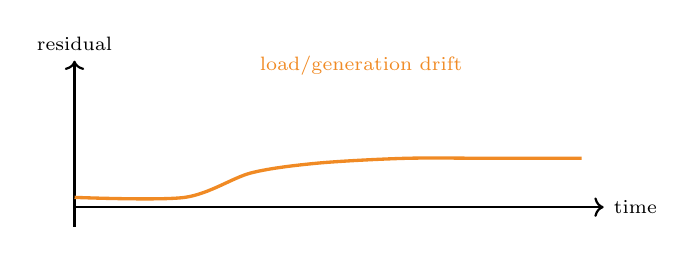
\begin{tikzpicture}[x=0.28cm,y=0.62cm]
  \draw[->,thick] (0,0) -- (24,0) node[right]{\scriptsize time};
  \draw[->,thick] (0,-0.4) -- (0,3.0) node[above]{\scriptsize residual};
  \draw[Orange,very thick,smooth] plot coordinates {(0,0.2)(5,0.2)(8,0.7)(11,0.9)(15,1.0)(19,1.0)(23,1.0)};
  \node[Orange] at (13,2.9) {\scriptsize load/generation drift};
\end{tikzpicture}
\end{column}
\begin{column}{0.46\textwidth}
\begin{block}{What the model sees}
Faults and switching tend to create a sharp innovation peak. Load and generation changes can create smaller but persistent residual deltas.
\end{block}
\begin{alertblock}{Used by final variant}
The selected localizer includes \code{rls\_kalman}; the non-selected \code{swing\_ekf} branch was tested but not used in the final route.
\end{alertblock}
\end{column}
\end{columns}
\end{frame}

% -------------------------------------------------------------------
\begin{frame}{Tested but not submitted: swing EKF idea}
\small
\begin{columns}[T,totalwidth=\textwidth]
\begin{column}{0.52\textwidth}
\begin{block}{Classical generator intuition}
\[
\dot{\delta}=\omega-\omega_0
\]
\[
M\dot{\omega}=P_m-P_e-D(\omega-\omega_0)
\]
\end{block}
\begin{exampleblock}{What the branch tried}
Use a light extended-Kalman style dynamic residual to capture frequency and angle swings after generation/load disturbances.
\end{exampleblock}
\end{column}
\begin{column}{0.44\textwidth}
\centering
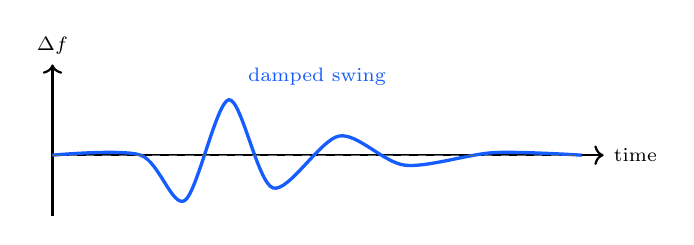
\begin{tikzpicture}[x=0.28cm,y=0.64cm]
  \draw[->,thick] (0,0) -- (25,0) node[right]{\scriptsize time};
  \draw[->,thick] (0,-1.2) -- (0,1.8) node[above]{\scriptsize $\Delta f$};
  \draw[Blue,very thick,smooth] plot coordinates {(0,0)(4,0)(6,-0.9)(8,1.1)(10,-0.65)(13,0.38)(16,-0.2)(20,0.05)(24,0.0)};
  \draw[Muted,dashed] (0,0) -- (24,0);
  \node[Blue] at (12,1.55) {\scriptsize damped swing};
\end{tikzpicture}
\vspace{2mm}
\begin{alertblock}{Why it was not final}
It improved some synthetic validation behavior but reduced RAW localization. The final route kept the simpler RLS/Kalman innovation block.
\end{alertblock}
\end{column}
\end{columns}
\end{frame}

% -------------------------------------------------------------------
\begin{frame}{Graph-temporal features}
\small
\begin{columns}[T,totalwidth=\textwidth]
\begin{column}{0.50\textwidth}
\begin{block}{What is computed}
\begin{itemize}
  \item PMU spread max/mean/p95.
  \item Time-to-peak range and standard deviation.
  \item Pairwise PMU differences.
  \item Pairwise PMU correlations.
  \item Pairwise time-to-peak differences.
  \item Weighted graph differences using electrical distance.
\end{itemize}
\end{block}
\end{column}
\begin{column}{0.46\textwidth}
\begin{exampleblock}{Why it helps localization}
The event origin leaves a spatial fingerprint: which PMU changed most, which changed first, and which pairs moved coherently.
\end{exampleblock}
\begin{alertblock}{Used most by}
Line outages and bus localization, where spatial pattern matters more than one local amplitude.
\end{alertblock}
\end{column}
\end{columns}
\end{frame}

% -------------------------------------------------------------------
\begin{frame}{Graph-temporal equations}
\small
\begin{columns}[T,totalwidth=\textwidth]
\begin{column}{0.52\textwidth}
\begin{block}{For signal $s$ and observed buses $\mathcal{B}$}
\[
\mathrm{spread}_s(t)=
\max_{b\in\mathcal{B}}\tilde{x}_{b,s}(t)
-
\min_{b\in\mathcal{B}}\tilde{x}_{b,s}(t)
\]
\[
\Delta_{ab,s}^{max}=\max_t|\tilde{x}_{a,s}(t)-\tilde{x}_{b,s}(t)|
\]
\[
\rho_{ab,s}=\mathrm{corr}(\tilde{x}_{a,s},\tilde{x}_{b,s})
\]
\[
\Delta t^{peak}_{ab,s}=
\left|t^{peak}_{a,s}-t^{peak}_{b,s}\right|
\]
\end{block}
\end{column}
\begin{column}{0.44\textwidth}
\begin{alertblock}{Electrical weighting}
\[
w_{ab}=\frac{1}{\max(d^{eff}_{ab},10^{-5})}
\]
\[
G_s^{max}=\max_{a<b}
w_{ab}\Delta_{ab,s}^{max}
\]
\end{alertblock}
\begin{exampleblock}{Feature names}
\code{GRAPH\_\_VA\_MAG\_\_pmu\_spread\_max}\\
\code{GRAPH\_\_Freq\_\_pair\_2\_39\_\_corr}\\
\code{GRAPH\_\_IA\_ANG\_\_weighted\_graph\_diff\_mean}
\end{exampleblock}
\end{column}
\end{columns}
\end{frame}

% -------------------------------------------------------------------
\begin{frame}{Graph-temporal localization illustration}
\small
\begin{columns}[T,totalwidth=\textwidth]
\begin{column}{0.56\textwidth}
\centering
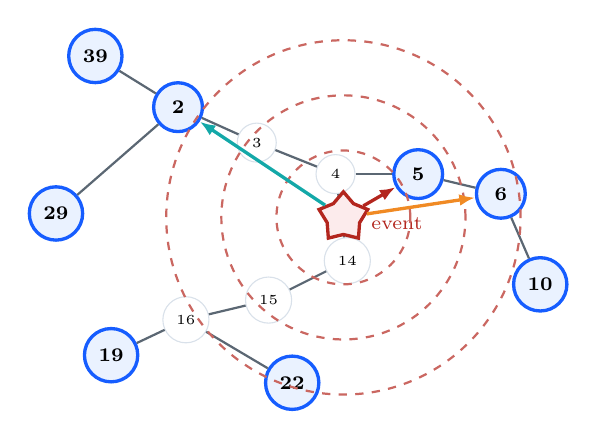
\begin{tikzpicture}[
  pmu/.style={circle,draw=Blue,fill=SoftBlue,very thick,minimum size=0.62cm,font=\scriptsize\bfseries},
  bus/.style={circle,draw=Line,fill=white,minimum size=0.42cm,font=\tiny},
  event/.style={star,star points=5,draw=Red,fill=SoftRed,very thick,minimum size=0.65cm},
  line/.style={draw=Muted,thick},
  pulse/.style={draw=Red!70,dashed,thick}
]
\node[pmu] (b2) at (0,1.7) {2};
\node[bus] (b3) at (1.0,1.25) {3};
\node[bus] (b4) at (2.0,0.85) {4};
\node[pmu] (b5) at (3.05,0.85) {5};
\node[pmu] (b6) at (4.1,0.6) {6};
\node[pmu] (b10) at (4.6,-0.55) {10};
\node[bus] (b14) at (2.15,-0.25) {14};
\node[bus] (b15) at (1.15,-0.75) {15};
\node[bus] (b16) at (0.1,-1.0) {16};
\node[pmu] (b19) at (-0.85,-1.45) {19};
\node[pmu] (b22) at (1.45,-1.8) {22};
\node[pmu] (b29) at (-1.55,0.35) {29};
\node[pmu] (b39) at (-1.05,2.35) {39};
\foreach \a/\b in {b39/b2,b2/b3,b3/b4,b4/b5,b5/b6,b6/b10,b4/b14,b14/b15,b15/b16,b16/b19,b16/b22,b2/b29} {
  \draw[line] (\a) -- (\b);
}
\node[event] (ev) at (2.1,0.3) {};
\node[Red] at (2.78,0.22) {\scriptsize event};
\draw[pulse] (ev) circle (0.85);
\draw[pulse] (ev) circle (1.55);
\draw[pulse] (ev) circle (2.25);
\draw[Red,very thick,-{Latex[length=2mm]}] (ev) -- (b5);
\draw[Orange,very thick,-{Latex[length=2mm]}] (ev) -- (b6);
\draw[Cyan,very thick,-{Latex[length=2mm]}] (ev) -- (b2);
\end{tikzpicture}
\end{column}
\begin{column}{0.40\textwidth}
\begin{block}{What a nearby PMU sees}
Larger amplitude, earlier peak, and stronger correlation with electrically close PMUs.
\end{block}
\begin{exampleblock}{What a remote PMU sees}
Smaller response, delayed peak, or lower pairwise coherence.
\end{exampleblock}
\begin{alertblock}{Line outage reading}
For Event 2, the localizer learns which line candidates match the current redistribution and graph-difference pattern.
\end{alertblock}
\end{column}
\end{columns}
\end{frame}

% -------------------------------------------------------------------
\begin{frame}{Why line outages need graph features}
\small
\begin{columns}[T,totalwidth=\textwidth]
\begin{column}{0.50\textwidth}
\centering
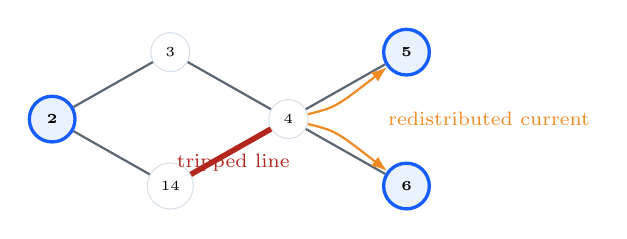
\begin{tikzpicture}[
  bus/.style={circle,draw=Line,fill=white,minimum size=0.48cm,font=\tiny},
  pmu/.style={circle,draw=Blue,fill=SoftBlue,very thick,minimum size=0.58cm,font=\tiny\bfseries},
  outage/.style={draw=Red,line width=2.0pt},
  line/.style={draw=Muted,thick},
  arrow/.style={-{Latex[length=2mm]},thick,draw=Orange}
]
\node[pmu] (a) at (0,0) {2};
\node[bus] (b) at (1.5,0.85) {3};
\node[bus] (c) at (3.0,0) {4};
\node[pmu] (d) at (4.5,0.85) {5};
\node[pmu] (e) at (4.5,-0.85) {6};
\node[bus] (f) at (1.5,-0.85) {14};
\draw[line] (a)--(b)--(c)--(d);
\draw[line] (c)--(e);
\draw[outage] (c)--(f);
\draw[line] (f)--(a);
\draw[arrow] (c) .. controls (3.6,0.15) .. (d);
\draw[arrow] (c) .. controls (3.6,-0.15) .. (e);
\node[Red] at (2.3,-0.55) {\scriptsize tripped line};
\node[Orange] at (5.55,0.0) {\scriptsize redistributed current};
\end{tikzpicture}
\end{column}
\begin{column}{0.46\textwidth}
\begin{block}{Electrical effect}
Opening one line changes current paths. Voltage may not collapse like a fault, but current magnitude, current angle, and pairwise PMU differences move in a structured way.
\end{block}
\begin{alertblock}{Feature consequence}
Event 2 benefits from graph differences, time-to-peak differences, and current-angle/current-magnitude signatures more than from a single largest voltage sag.
\end{alertblock}
\end{column}
\end{columns}
\end{frame}

% -------------------------------------------------------------------
\begin{frame}{Final selected feature variant}
\small
\begin{columns}[T,totalwidth=\textwidth]
\begin{column}{0.46\textwidth}
\begin{block}{Selected}
\[
\texttt{base\_v2 + rolling + rls\_kalman + graph\_temporal}
\]
\[
n_{\mathrm{features}} = 45{,}162
\]
\end{block}
\end{column}
\begin{column}{0.50\textwidth}
\begin{alertblock}{Not selected}
\begin{itemize}
  \item \code{algebraic\_residual\_v4}: matched RAW but did not improve it.
  \item \code{swing\_ekf}: improved SIM slightly, reduced RAW localization.
  \item oracle topology ranker: better RAW, but not deployable.
\end{itemize}
\end{alertblock}
\end{column}
\end{columns}
\vspace{2mm}
\begin{exampleblock}{Selection criterion}
Highest RAW0001 localization among production-feasible variants while keeping strong synthetic validation performance.
\end{exampleblock}
\end{frame}

% -------------------------------------------------------------------
\section{Hierarchical ML Method}

\begin{frame}[plain]{}
\begin{tikzpicture}[remember picture,overlay]
  \fill[Navy] (current page.south west) rectangle (current page.north east);
  \node[anchor=west] at ($(current page.west)+(0.8,0.6)$) {\color{Cyan}\Large Section 5};
  \node[anchor=west,text width=0.82\paperwidth] at ($(current page.west)+(0.8,-0.15)$) {\color{white}\Huge\bfseries Hierarchical ML Method};
  \node[anchor=south east] at ($(current page.south east)+(-0.4,0.35)$) {\sgsmalogo[1.0cm]};
\end{tikzpicture}
\end{frame}

% -------------------------------------------------------------------
\begin{frame}{Why ExtraTrees?}
\small
\begin{columns}[T,totalwidth=\textwidth]
\begin{column}{0.47\textwidth}
\begin{block}{Pipeline}
\[
X \rightarrow \mathrm{SimpleImputer(median)} \rightarrow \mathrm{ExtraTreesClassifier}
\]
\end{block}
\begin{exampleblock}{Imputation}
Median imputation handles NaNs and missing feature values without requiring a complex preprocessing model.
\end{exampleblock}
\end{column}
\begin{column}{0.49\textwidth}
\begin{alertblock}{Why ExtraTrees worked well}
\begin{itemize}
  \item Handles many features.
  \item Does not require scaling.
  \item Captures nonlinear interactions.
  \item Tolerates noisy/outlier-prone features.
  \item Fast enough for repeated experiments.
\end{itemize}
\end{alertblock}
\end{column}
\end{columns}
\end{frame}

% -------------------------------------------------------------------
\begin{frame}{ExtraTrees decision rule}
\small
\begin{columns}[T,totalwidth=\textwidth]
\begin{column}{0.50\textwidth}
\begin{block}{Ensemble probability}
\[
\hat{p}(c\mid x)=
\frac{1}{M}\sum_{m=1}^{M}
\mathbb{1}\left[h_m(x)=c\right]
\]
\[
\hat{c}=\arg\max_c \hat{p}(c\mid x)
\]
\end{block}
\begin{exampleblock}{What makes ExtraTrees different}
Each tree uses randomized split candidates. That reduces variance and works well when many engineered features are redundant but useful.
\end{exampleblock}
\end{column}
\begin{column}{0.46\textwidth}
\centering
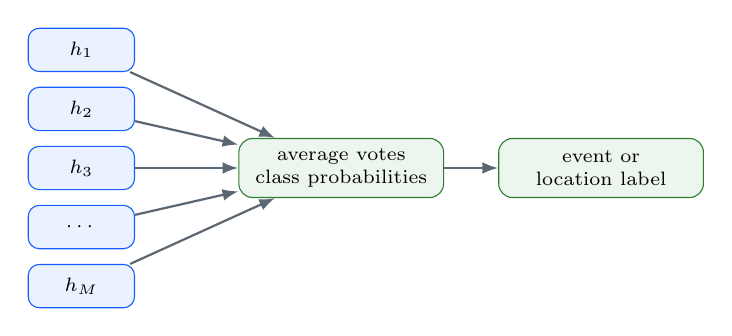
\begin{tikzpicture}[
  tree/.style={rounded corners=4pt,draw=Blue,fill=SoftBlue,minimum width=1.35cm,minimum height=0.55cm,font=\scriptsize},
  vote/.style={rounded corners=5pt,draw=Green,fill=SoftGreen,minimum width=2.6cm,minimum height=0.75cm,align=center,font=\scriptsize},
  arrow/.style={-{Latex[length=2mm]},thick,draw=Muted}
]
\node[tree] (t1) at (0,1.5) {$h_1$};
\node[tree] (t2) at (0,0.75) {$h_2$};
\node[tree] (t3) at (0,0.0) {$h_3$};
\node[tree] (t4) at (0,-0.75) {$\cdots$};
\node[tree] (t5) at (0,-1.5) {$h_M$};
\node[vote] (v) at (3.3,0) {average votes\\class probabilities};
\node[vote] (o) at (6.6,0) {event or\\location label};
\foreach \t in {t1,t2,t3,t4,t5} {
  \draw[arrow] (\t) -- (v);
}
\draw[arrow] (v) -- (o);
\end{tikzpicture}
\vspace{2mm}
\begin{alertblock}{Pipeline detail}
Before the forest, missing values are replaced by the training median of each feature column.
\end{alertblock}
\end{column}
\end{columns}
\end{frame}

% -------------------------------------------------------------------
\begin{frame}{Final model components}
\small
\centering
\begin{tabular}{p{0.30\textwidth}p{0.31\textwidth}p{0.27\textwidth}}
\toprule
\textbf{Model artifact} & \textbf{Role} & \textbf{Output}\\
\midrule
\code{physical\_event\_classifier.joblib} & Main physical event classifier & 0,1,2,3,4,8\\
\code{bad\_data\_detector.joblib} & Event 7 detector & bad / not bad\\
\code{missing\_composition\_detector.joblib} & Event 5/6 support & missing composition\\
\code{final\_dynamic\_localizers.joblib} & Typed localizers & BUS, LINE, PMU\\
\code{hierarchical\_model\_config.json} & Rule thresholds & final event logic\\
\bottomrule
\end{tabular}
\end{frame}

% -------------------------------------------------------------------
\begin{frame}{Hierarchical event logic}
\centering
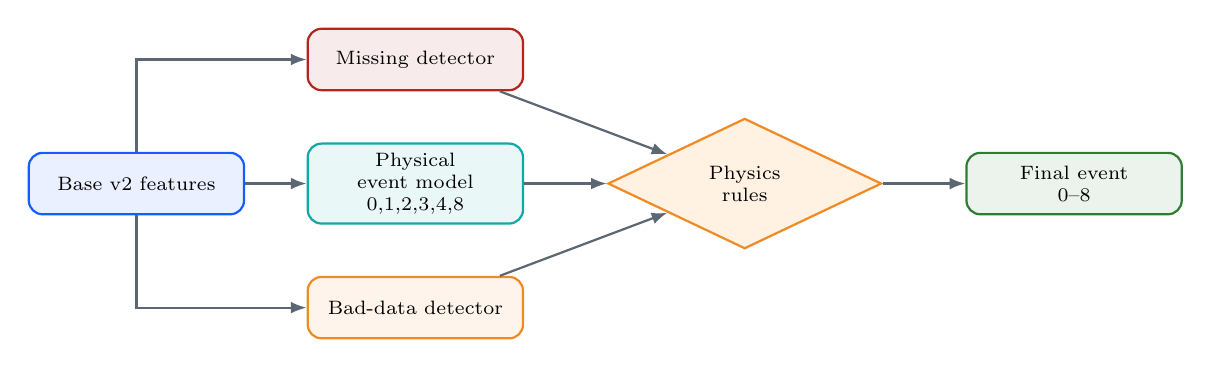
\begin{tikzpicture}[
  node distance=0.65cm and 0.78cm,
  boxblue/.style={rounded corners=5pt,draw=Blue,fill=Blue!9,thick,text width=2.5cm,minimum height=0.78cm,align=center,font=\scriptsize},
  boxcyan/.style={rounded corners=5pt,draw=Cyan,fill=Cyan!9,thick,text width=2.5cm,minimum height=0.78cm,align=center,font=\scriptsize},
  boxgreen/.style={rounded corners=5pt,draw=Green,fill=Green!9,thick,text width=2.5cm,minimum height=0.78cm,align=center,font=\scriptsize},
  boxorange/.style={rounded corners=5pt,draw=Orange,fill=Orange!9,thick,text width=2.5cm,minimum height=0.78cm,align=center,font=\scriptsize},
  boxred/.style={rounded corners=5pt,draw=Red,fill=Red!9,thick,text width=2.5cm,minimum height=0.78cm,align=center,font=\scriptsize},
  gate/.style={diamond,aspect=2.1,draw=Orange,fill=SoftOrange,thick,text width=1.8cm,align=center,font=\scriptsize},
  arrow/.style={-{Latex[length=2mm]},thick,draw=Muted}
]
\node[boxblue] (x) {Base v2 features};
\node[boxcyan,right=of x] (phys) {Physical event model\\0,1,2,3,4,8};
\node[boxred,above=of phys] (miss) {Missing detector};
\node[boxorange,below=of phys] (bad) {Bad-data detector};
\node[gate,right=1.05cm of phys] (rules) {Physics\\rules};
\node[boxgreen,right=1.05cm of rules] (event) {Final event\\0--8};
\draw[arrow] (x) -- (phys);
\draw[arrow] (x) |- (miss);
\draw[arrow] (x) |- (bad);
\draw[arrow] (phys) -- (rules);
\draw[arrow] (miss) -- (rules);
\draw[arrow] (bad) -- (rules);
\draw[arrow] (rules) -- (event);
\end{tikzpicture}
\vspace{4mm}
\begin{block}{Why hierarchical?}
Missing data and bad data are measurement phenomena. They should not be forced into the same flat classifier decision as physical grid events.
\end{block}
\end{frame}

% -------------------------------------------------------------------
\begin{frame}{Physics rule guards}
\small
\begin{columns}[T,totalwidth=\textwidth]
\begin{column}{0.50\textwidth}
\begin{block}{Fault-like}
\[
V_{\mathrm{span}} \ge 50{,}000
\]
\[
\max |dV/dt| \ge 500{,}000
\]
\end{block}
\begin{block}{Line-outage-like}
\[
I_{\mathrm{span}} \ge 500
\]
\[
\max |dI/dt| \ge 3{,}000
\]
\[
V_{\mathrm{span}} \le 50{,}000
\]
\end{block}
\end{column}
\begin{column}{0.46\textwidth}
\begin{alertblock}{Missing-like}
\[
\mathrm{data\_present\_fraction}<0.999
\]
or high NaN/gap features.
\end{alertblock}
\begin{alertblock}{Bad-data-like}
\[
\mathrm{single\_signal\_score}\ge 200{,}000
\]
\[
\mathrm{single\_signal\_ratio}\ge 3.0
\]
\end{alertblock}
\end{column}
\end{columns}
\end{frame}

% -------------------------------------------------------------------
\begin{frame}{Rule engine as a decision tree}
\small
\centering
\resizebox{!}{0.48\textheight}{%
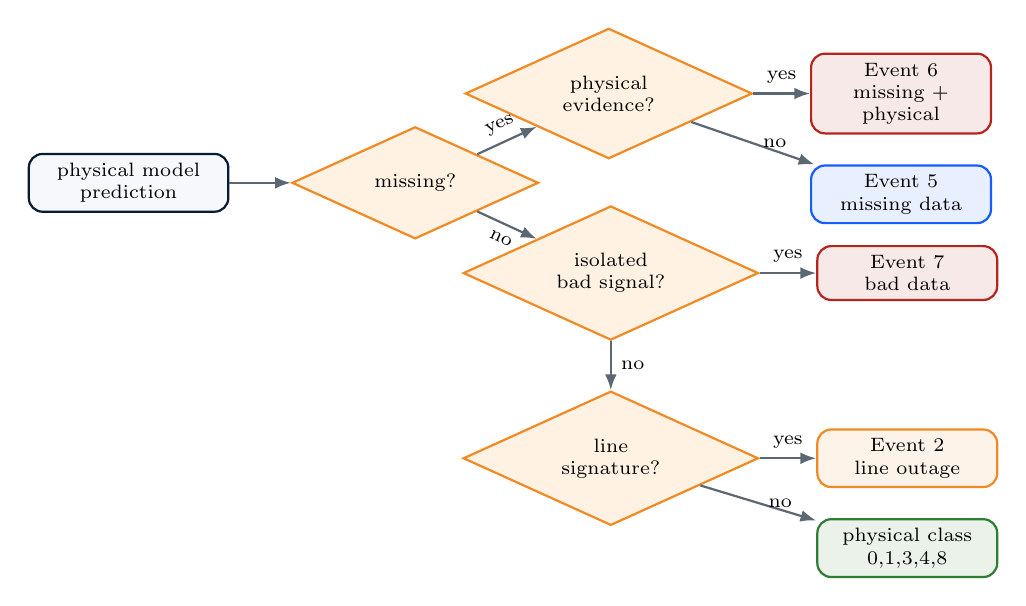
\begin{tikzpicture}[
  node distance=0.55cm and 0.78cm,
  decision/.style={diamond,aspect=2.2,draw=Orange,fill=SoftOrange,thick,text width=1.9cm,align=center,font=\scriptsize},
  leafred/.style={rounded corners=5pt,draw=Red,fill=Red!10,thick,text width=2.05cm,minimum height=0.68cm,align=center,font=\scriptsize},
  leafblue/.style={rounded corners=5pt,draw=Blue,fill=Blue!10,thick,text width=2.05cm,minimum height=0.68cm,align=center,font=\scriptsize},
  leaforange/.style={rounded corners=5pt,draw=Orange,fill=Orange!10,thick,text width=2.05cm,minimum height=0.68cm,align=center,font=\scriptsize},
  leafgreen/.style={rounded corners=5pt,draw=Green,fill=Green!10,thick,text width=2.05cm,minimum height=0.68cm,align=center,font=\scriptsize},
  proc/.style={rounded corners=5pt,draw=Navy,fill=Paper,thick,text width=2.3cm,minimum height=0.68cm,align=center,font=\scriptsize},
  arrow/.style={-{Latex[length=2mm]},thick,draw=Muted}
]
\node[proc] (phys) {physical model\\prediction};
\node[decision,right=of phys] (miss) {missing?};
\node[decision,above right=0.35cm and 0.75cm of miss] (physe) {physical\\evidence?};
\node[leafred,right=0.72cm of physe] (e6) {Event 6\\missing + physical};
\node[leafblue,below=0.38cm of e6] (e5) {Event 5\\missing data};
\node[decision,below right=0.35cm and 0.75cm of miss] (bad) {isolated\\bad signal?};
\node[leafred,right=0.72cm of bad] (e7) {Event 7\\bad data};
\node[decision,below=0.62cm of bad] (line) {line\\signature?};
\node[leaforange,right=0.72cm of line] (e2) {Event 2\\line outage};
\node[leafgreen,below=0.38cm of e2] (physout) {physical class\\0,1,3,4,8};
\draw[arrow] (phys) -- (miss);
\draw[arrow] (miss) -- node[above,sloped]{\scriptsize yes} (physe);
\draw[arrow] (physe) -- node[above]{\scriptsize yes} (e6);
\draw[arrow] (physe) -- node[right]{\scriptsize no} (e5);
\draw[arrow] (miss) -- node[below,sloped]{\scriptsize no} (bad);
\draw[arrow] (bad) -- node[above]{\scriptsize yes} (e7);
\draw[arrow] (bad) -- node[right]{\scriptsize no} (line);
\draw[arrow] (line) -- node[above]{\scriptsize yes} (e2);
\draw[arrow] (line) -- node[right]{\scriptsize no} (physout);
\end{tikzpicture}%
}
\vspace{0.5mm}
\begin{block}{What this diagram leaves out}
The implementation also uses confidence gates so weak physical predictions do not override strong missing or bad-data evidence.
\end{block}
\end{frame}

% -------------------------------------------------------------------
\begin{frame}{Final event decision in plain English}
\small
\begin{enumerate}
  \item Predict the physical event class using the physical ExtraTrees model.
  \item Compute physical confidence from predicted probabilities.
  \item Check missing-data evidence from data-quality features.
  \item Check bad-data evidence from single-signal anomaly features.
  \item Use fault and line-outage guards to correct ambiguous physical predictions.
  \item If missing is present, decide Event 5 vs Event 6 using physical evidence.
  \item If isolated bad-data evidence dominates, assign Event 7.
\end{enumerate}
\vspace{2mm}
\begin{alertblock}{Interpretability benefit}
The final decision can be defended physically: voltage fault, current redistribution, missing data, or isolated sensor corruption.
\end{alertblock}
\end{frame}

% -------------------------------------------------------------------
\section{Event-by-Event Interpretation}

\begin{frame}[plain]{}
\begin{tikzpicture}[remember picture,overlay]
  \fill[Navy] (current page.south west) rectangle (current page.north east);
  \node[anchor=west] at ($(current page.west)+(0.8,0.6)$) {\color{Cyan}\Large Section 6};
  \node[anchor=west,text width=0.82\paperwidth] at ($(current page.west)+(0.8,-0.15)$) {\color{white}\Huge\bfseries Event-by-Event Interpretation};
  \node[anchor=south east] at ($(current page.south east)+(-0.4,0.35)$) {\sgsmalogo[1.0cm]};
\end{tikzpicture}
\end{frame}

% -------------------------------------------------------------------
\begin{frame}{Event 1: fault}
\small
\begin{columns}[T,totalwidth=\textwidth]
\begin{column}{0.48\textwidth}
\begin{block}{Main evidence}
\begin{itemize}
  \item Voltage magnitude span.
  \item Voltage derivative.
  \item Robust z-score in voltage channels.
  \item Early segment changes.
  \item Cross-PMU severity pattern.
\end{itemize}
\end{block}
\end{column}
\begin{column}{0.48\textwidth}
\begin{alertblock}{Manual recipe}
\begin{enumerate}
  \item Build baseline from pre-event voltage.
  \item Detect large voltage sag/transient.
  \item Reject missing-only and bad-data-only cases.
  \item Localize to BUS using spatial severity.
\end{enumerate}
\end{alertblock}
\end{column}
\end{columns}
\end{frame}

% -------------------------------------------------------------------
\begin{frame}{Event 2: line outage}
\small
\begin{columns}[T,totalwidth=\textwidth]
\begin{column}{0.48\textwidth}
\begin{block}{Main evidence}
\begin{itemize}
  \item Current magnitude span.
  \item Current derivative.
  \item Current-angle changes.
  \item Voltage span not as extreme as a fault.
  \item Graph-temporal pairwise PMU differences.
\end{itemize}
\end{block}
\end{column}
\begin{column}{0.48\textwidth}
\begin{alertblock}{Manual recipe}
\begin{enumerate}
  \item Look for current redistribution.
  \item Guard against fault-like voltage collapse.
  \item Use graph features to score candidate lines.
  \item Localize to LINE.
\end{enumerate}
\end{alertblock}
\end{column}
\end{columns}
\end{frame}

% -------------------------------------------------------------------
\begin{frame}{Event 3: generation change}
\small
\begin{columns}[T,totalwidth=\textwidth]
\begin{column}{0.48\textwidth}
\begin{block}{Main evidence}
\begin{itemize}
  \item Frequency shift.
  \item ROCOF response.
  \item Active-power proxy change.
  \item Late/pre sustained delta.
  \item RLS/Kalman residuals.
\end{itemize}
\end{block}
\end{column}
\begin{column}{0.48\textwidth}
\begin{exampleblock}{Physical explanation}
Generation changes disturb the active-power balance. The grid response is often visible in frequency, ROCOF, and power proxy rather than only voltage magnitude.
\end{exampleblock}
\end{column}
\end{columns}
\end{frame}

% -------------------------------------------------------------------
\begin{frame}{Event 4: load change}
\small
\begin{columns}[T,totalwidth=\textwidth]
\begin{column}{0.48\textwidth}
\begin{block}{Main evidence}
\begin{itemize}
  \item Current magnitude level shift.
  \item Active/reactive power proxy.
  \item Power-factor angle.
  \item Late segment persistence.
  \item Less abrupt than a fault.
\end{itemize}
\end{block}
\end{column}
\begin{column}{0.48\textwidth}
\begin{exampleblock}{Physical explanation}
Load changes alter consumption. They often appear as sustained current and power-proxy shifts with less violent voltage transients.
\end{exampleblock}
\end{column}
\end{columns}
\end{frame}

% -------------------------------------------------------------------
\begin{frame}{Events 5 and 6: missing data}
\small
\begin{columns}[T,totalwidth=\textwidth]
\begin{column}{0.49\textwidth}
\begin{block}{Event 5: missing data}
\begin{itemize}
  \item DATA\_PRESENT drops.
  \item Timestamp gaps grow.
  \item NaN fraction increases.
  \item No strong physical event evidence.
\end{itemize}
\end{block}
\end{column}
\begin{column}{0.47\textwidth}
\begin{alertblock}{Event 6: missing + physical}
\begin{itemize}
  \item Missing-data evidence exists.
  \item Physical classifier is not normal.
  \item Physical confidence is sufficient.
  \item Location may be BUS or LINE depending on physical event.
\end{itemize}
\end{alertblock}
\end{column}
\end{columns}
\end{frame}

% -------------------------------------------------------------------
\begin{frame}{Event 7: bad data}
\small
\begin{columns}[T,totalwidth=\textwidth]
\begin{column}{0.48\textwidth}
\begin{block}{Main evidence}
\begin{itemize}
  \item One signal has extreme robust z-score.
  \item Top anomaly is much larger than second anomaly.
  \item Other PMUs/channels remain coherent.
  \item Missing features do not dominate.
\end{itemize}
\end{block}
\end{column}
\begin{column}{0.48\textwidth}
\begin{alertblock}{Localizer}
Event 7 localizes to PMU, not BUS or LINE. The object that failed is the measurement device/channel source.
\end{alertblock}
\end{column}
\end{columns}
\end{frame}

% -------------------------------------------------------------------
\begin{frame}{Event 8: mixed proxy}
\small
\begin{block}{Main evidence}
Event 8 captures cases with physical evidence that does not cleanly fit fault, line outage, generation change, or load change.
\end{block}
\begin{columns}[T,totalwidth=\textwidth]
\begin{column}{0.48\textwidth}
\begin{exampleblock}{Useful features}
\begin{itemize}
  \item Power proxy.
  \item Rolling dynamics.
  \item RLS/Kalman residuals.
  \item Graph-temporal pattern.
\end{itemize}
\end{exampleblock}
\end{column}
\begin{column}{0.48\textwidth}
\begin{alertblock}{Routing}
The final runtime routes Event 8 to a BUS localizer because it represents a physical-grid signature rather than a PMU-only failure.
\end{alertblock}
\end{column}
\end{columns}
\end{frame}

% -------------------------------------------------------------------
\section{Localization}

\begin{frame}[plain]{}
\begin{tikzpicture}[remember picture,overlay]
  \fill[Navy] (current page.south west) rectangle (current page.north east);
  \node[anchor=west] at ($(current page.west)+(0.8,0.6)$) {\color{Cyan}\Large Section 7};
  \node[anchor=west,text width=0.82\paperwidth] at ($(current page.west)+(0.8,-0.15)$) {\color{white}\Huge\bfseries Localization};
  \node[anchor=south east] at ($(current page.south east)+(-0.4,0.35)$) {\sgsmalogo[1.0cm]};
\end{tikzpicture}
\end{frame}

% -------------------------------------------------------------------
\begin{frame}{Typed localization routing}
\small
\begin{columns}[T,totalwidth=\textwidth]
\begin{column}{0.48\textwidth}
\begin{block}{Event routing}
\begin{tabular}{cl}
\toprule
Event & Localizer type\\
\midrule
1 fault & BUS\\
2 line outage & LINE\\
3 generation change & BUS\\
4 load change & BUS\\
5 missing data & PMU\\
6 missing + physical & BUS or LINE\\
7 bad data & PMU\\
8 mixed proxy & BUS\\
\bottomrule
\end{tabular}
\end{block}
\end{column}
\begin{column}{0.48\textwidth}
\begin{alertblock}{Routing reason}
A line outage, a bus fault, and a bad PMU are different localization problems. A single flat location classifier would mix incompatible targets.
\end{alertblock}
\end{column}
\end{columns}
\end{frame}

% -------------------------------------------------------------------
\begin{frame}{Three location spaces}
\small
\centering
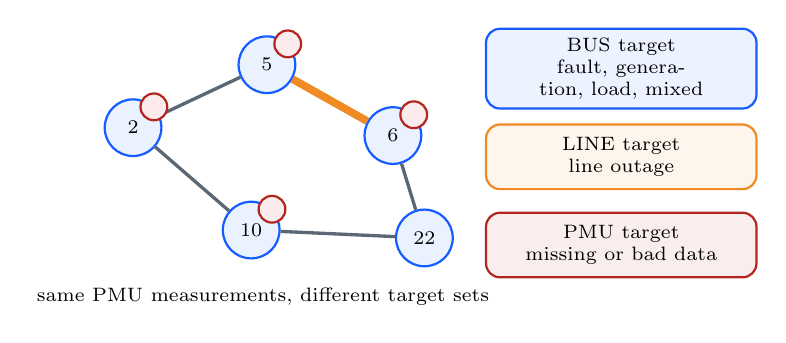
\begin{tikzpicture}[
  bus/.style={circle,draw=Blue,fill=SoftBlue,thick,minimum size=0.72cm,font=\scriptsize},
  pmu/.style={circle,draw=Red,fill=SoftRed,thick,minimum size=0.34cm},
  line/.style={draw=Muted,line width=1.2pt},
  label/.style={font=\scriptsize,align=center},
  boxblue/.style={rounded corners=5pt,draw=Blue,fill=Blue!8,thick,text width=3.2cm,minimum height=0.82cm,align=center,font=\scriptsize},
  boxorange/.style={rounded corners=5pt,draw=Orange,fill=Orange!8,thick,text width=3.2cm,minimum height=0.82cm,align=center,font=\scriptsize},
  boxred/.style={rounded corners=5pt,draw=Red,fill=Red!8,thick,text width=3.2cm,minimum height=0.82cm,align=center,font=\scriptsize}
]
\node[bus] (b2) at (0,1.4) {2};
\node[bus] (b5) at (1.7,2.2) {5};
\node[bus] (b6) at (3.3,1.3) {6};
\node[bus] (b10) at (1.5,0.1) {10};
\node[bus] (b22) at (3.7,0.0) {22};
\draw[line] (b2) -- (b5);
\draw[line,Orange,line width=2.8pt] (b5) -- (b6);
\draw[line] (b2) -- (b10);
\draw[line] (b10) -- (b22);
\draw[line] (b6) -- (b22);
\node[pmu] at (b2.north east) {};
\node[pmu] at (b5.north east) {};
\node[pmu] at (b6.north east) {};
\node[pmu] at (b10.north east) {};
\node[boxblue] at (6.2,2.15) {BUS target\\fault, generation, load, mixed};
\node[boxorange] at (6.2,1.03) {LINE target\\line outage};
\node[boxred] at (6.2,-0.09) {PMU target\\missing or bad data};
\node[label] at (1.65,-0.75) {same PMU measurements, different target sets};
\end{tikzpicture}
\vspace{2mm}
\begin{block}{How to explain it}
The location column does not always mean a bus. Its meaning depends on the event class.
\end{block}
\end{frame}

% -------------------------------------------------------------------
\begin{frame}{Final localizer models}
\small
\begin{block}{Localizer keys in the final dynamic bundle}
\centering
\code{BUS}, \code{BUS:event1}, \code{BUS:event3}, \code{BUS:event4}, \code{BUS:event8},\\
\code{LINE}, \code{LINE:event2}, \code{PMU}
\end{block}
\begin{exampleblock}{Model family}
Each localizer is a median-imputed ExtraTrees pipeline trained on base + dynamic features.
\end{exampleblock}
\begin{alertblock}{Final Top-1}
\code{use\_hybrid\_top1 = false}. The final submitted Top-1 location uses the validated typed ML localizers, not the hybrid/oracle branch.
\end{alertblock}
\end{frame}

% -------------------------------------------------------------------
\begin{frame}{What the localizer learns}
\small
\begin{columns}[T,totalwidth=\textwidth]
\begin{column}{0.32\textwidth}
\begin{block}{BUS}
\begin{itemize}
  \item nearest severe response,
  \item voltage/frequency signature,
  \item graph spread pattern.
\end{itemize}
\end{block}
\end{column}
\begin{column}{0.32\textwidth}
\begin{block}{LINE}
\begin{itemize}
  \item current redistribution,
  \item pairwise PMU differences,
  \item topology-aware graph signature.
\end{itemize}
\end{block}
\end{column}
\begin{column}{0.32\textwidth}
\begin{block}{PMU}
\begin{itemize}
  \item missing run,
  \item isolated bad channel,
  \item local data-quality failure.
\end{itemize}
\end{block}
\end{column}
\end{columns}
\vspace{2mm}
\begin{alertblock}{Location signal}
Location is inferred from the pattern of who saw the disturbance, how strongly, and how early.
\end{alertblock}
\end{frame}

% -------------------------------------------------------------------
\begin{frame}{Localizer inference equation}
\small
\begin{columns}[T,totalwidth=\textwidth]
\begin{column}{0.52\textwidth}
\begin{block}{Feature vector for location}
\[
x_{\mathrm{loc}}=
\left[
x_{\mathrm{base\_v2}},\
x_{\mathrm{rolling}},\
x_{\mathrm{rls/kalman}},\
x_{\mathrm{graph}}
\right]
\]
\[
\hat{e}=H(x_{\mathrm{base\_v2}})
\]
\[
\hat{\ell}=L_{g(\hat{e})}(x_{\mathrm{loc}})
\]
\end{block}
\begin{exampleblock}{Route function}
\[
g(e)\in\{\mathrm{BUS},\mathrm{LINE},\mathrm{PMU}\}
\]
\end{exampleblock}
\end{column}
\begin{column}{0.44\textwidth}
\centering
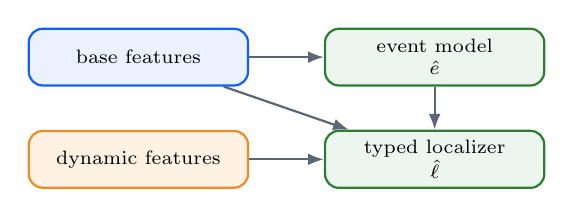
\begin{tikzpicture}[
  node distance=0.55cm,
  box/.style={rounded corners=5pt,draw=Blue,fill=SoftBlue,thick,text width=2.55cm,minimum height=0.72cm,align=center,font=\scriptsize},
  box2/.style={rounded corners=5pt,draw=Orange,fill=SoftOrange,thick,text width=2.55cm,minimum height=0.72cm,align=center,font=\scriptsize},
  box3/.style={rounded corners=5pt,draw=Green,fill=SoftGreen,thick,text width=2.55cm,minimum height=0.72cm,align=center,font=\scriptsize},
  arrow/.style={-{Latex[length=2mm]},thick,draw=Muted}
]
\node[box] (base) {base features};
\node[box2,below=of base] (dyn) {dynamic features};
\node[box3,right=0.95cm of base] (event) {event model\\$\hat{e}$};
\node[box3,right=0.95cm of dyn] (loc) {typed localizer\\$\hat{\ell}$};
\draw[arrow] (base) -- (event);
\draw[arrow] (event) -- (loc);
\draw[arrow] (base) -- (loc);
\draw[arrow] (dyn) -- (loc);
\end{tikzpicture}
\vspace{2mm}
\begin{alertblock}{Reason for two feature views}
The event classifier is stable with base features. The localizer gets the larger dynamic vector because location depends on propagation and topology.
\end{alertblock}
\end{column}
\end{columns}
\end{frame}

% -------------------------------------------------------------------
\begin{frame}{BUS, LINE, and PMU targets}
\small
\begin{columns}[T,totalwidth=\textwidth]
\begin{column}{0.32\textwidth}
\begin{block}{BUS}
\[
\mathcal{Y}_{BUS}=\{1,\dots,39\}
\]
Target is the electrical bus where the physical disturbance is assigned.
\end{block}
\end{column}
\begin{column}{0.32\textwidth}
\begin{block}{LINE}
\[
\mathcal{Y}_{LINE}=\{(i,j):(i,j)\in\mathcal{E}\}
\]
Target is a branch in the IEEE 39 topology.
\end{block}
\end{column}
\begin{column}{0.32\textwidth}
\begin{block}{PMU}
\[
\mathcal{Y}_{PMU}=\{2,5,6,10,19,22,29,39\}
\]
Target is the observed device affected by missing or bad data.
\end{block}
\end{column}
\end{columns}
\vspace{2mm}
\centering
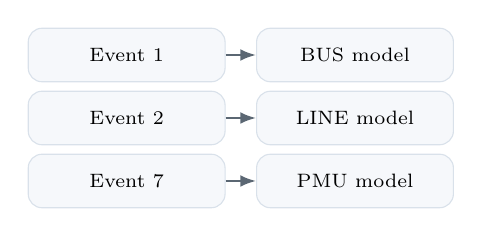
\begin{tikzpicture}[
  target/.style={rounded corners=5pt,draw=Line,fill=Paper,minimum width=2.5cm,minimum height=0.68cm,align=center,font=\scriptsize},
  arrow/.style={-{Latex[length=2mm]},thick,draw=Muted}
]
\node[target] (e1) at (0,0) {Event 1};
\node[target] (bus) at (2.9,0) {BUS model};
\node[target] (e2) at (0,-0.8) {Event 2};
\node[target] (line) at (2.9,-0.8) {LINE model};
\node[target] (e7) at (0,-1.6) {Event 7};
\node[target] (pmu) at (2.9,-1.6) {PMU model};
\draw[arrow] (e1) -- (bus);
\draw[arrow] (e2) -- (line);
\draw[arrow] (e7) -- (pmu);
\end{tikzpicture}
\end{frame}

% -------------------------------------------------------------------
\begin{frame}{What makes localization harder than classification}
\small
\begin{columns}[T,totalwidth=\textwidth]
\begin{column}{0.55\textwidth}
\centering
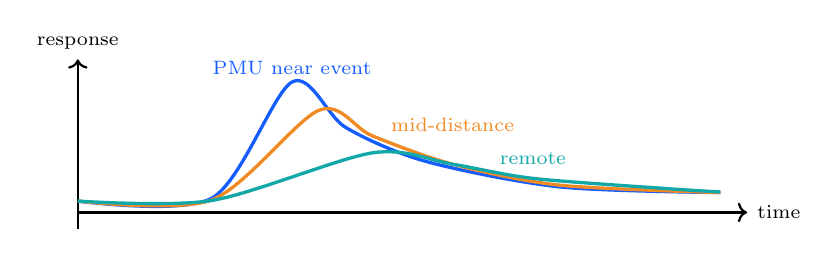
\begin{tikzpicture}[x=0.34cm,y=0.72cm]
  \draw[->,thick] (0,0) -- (25,0) node[right]{\scriptsize time};
  \draw[->,thick] (0,-0.3) -- (0,2.7) node[above]{\scriptsize response};
  \draw[Blue,very thick,smooth] plot coordinates {(0,0.2)(5,0.25)(8,2.3)(10,1.5)(13,0.9)(18,0.45)(24,0.35)};
  \draw[Orange,very thick,smooth] plot coordinates {(0,0.2)(5,0.22)(9,1.8)(11,1.35)(14,0.85)(18,0.48)(24,0.35)};
  \draw[Cyan,very thick,smooth] plot coordinates {(0,0.2)(5,0.21)(11,1.05)(14,0.85)(17,0.60)(22,0.42)(24,0.36)};
  \node[Blue] at (8,2.55) {\scriptsize PMU near event};
  \node[Orange] at (14,1.55) {\scriptsize mid-distance};
  \node[Cyan] at (17,0.95) {\scriptsize remote};
\end{tikzpicture}
\end{column}
\begin{column}{0.41\textwidth}
\begin{block}{Classification}
Often needs to know whether the pattern resembles a fault, outage, load change, missing data, or bad data.
\end{block}
\begin{alertblock}{Localization}
Needs the finer spatial ordering: which PMU changed first, which changed most, and which candidate location best explains that pattern.
\end{alertblock}
\end{column}
\end{columns}
\end{frame}

% -------------------------------------------------------------------
\section{Training, Validation, and Results}

\begin{frame}[plain]{}
\begin{tikzpicture}[remember picture,overlay]
  \fill[Navy] (current page.south west) rectangle (current page.north east);
  \node[anchor=west] at ($(current page.west)+(0.8,0.6)$) {\color{Cyan}\Large Section 8};
  \node[anchor=west,text width=0.82\paperwidth] at ($(current page.west)+(0.8,-0.15)$) {\color{white}\Huge\bfseries Training, Validation, and Results};
  \node[anchor=south east] at ($(current page.south east)+(-0.4,0.35)$) {\sgsmalogo[1.0cm]};
\end{tikzpicture}
\end{frame}

% -------------------------------------------------------------------
\begin{frame}{Training data and split}
\small
\begin{columns}[T,totalwidth=\textwidth]
\begin{column}{0.48\textwidth}
\begin{block}{Training sources}
\begin{itemize}
  \item Synthetic SGSMA scenarios.
  \item Base features: \code{factory\_features\_v2.csv}.
  \item Dynamic features: \code{dynamic\_features\_v3.csv}.
  \item Random state: \code{20260503}.
\end{itemize}
\end{block}
\end{column}
\begin{column}{0.48\textwidth}
\begin{exampleblock}{Validation}
\begin{itemize}
  \item 30\% stratified SIM holdout.
  \item RAW0001 transfer validation.
  \item Metrics: detector, classifier, macro-F1, localization.
\end{itemize}
\end{exampleblock}
\end{column}
\end{columns}
\vspace{2mm}
\begin{alertblock}{Generalization principle}
RAW labels were used for validation and analysis, not to train the final production-feasible submission path.
\end{alertblock}
\end{frame}

% -------------------------------------------------------------------
\begin{frame}{Final metrics}
\small
\begin{columns}[T,totalwidth=\textwidth]
\begin{column}{0.49\textwidth}
\begin{block}{SIM holdout}
\centering
\begin{tabular}{lr}
\toprule
Metric & Score\\
\midrule
Detector accuracy & 0.9693\\
Classifier accuracy & 0.9673\\
Classifier macro-F1 & 0.9598\\
Localizer Top-1 & 0.8524\\
\bottomrule
\end{tabular}
\end{block}
\end{column}
\begin{column}{0.47\textwidth}
\begin{alertblock}{RAW0001}
\centering
\begin{tabular}{lr}
\toprule
Metric & Score\\
\midrule
Detector accuracy & 1.0000\\
Classifier accuracy & 1.0000\\
Classifier macro-F1 & 1.0000\\
Localizer Top-1 & 0.6667\\
\bottomrule
\end{tabular}
\end{alertblock}
\end{column}
\end{columns}
\vspace{2mm}
\begin{exampleblock}{Interpretation}
Detection and classification transferred perfectly on RAW0001; localization remained the hard part.
\end{exampleblock}
\end{frame}

% -------------------------------------------------------------------
\begin{frame}{Why the final variant was selected}
\small
\begin{block}{Selected variant}
\[
\texttt{base\_v2 + rolling + rls\_kalman + graph\_temporal}
\]
\end{block}
\begin{columns}[T,totalwidth=\textwidth]
\begin{column}{0.48\textwidth}
\begin{exampleblock}{Strength}
\begin{itemize}
  \item Strong SIM performance.
  \item Best RAW localization tier among deployable variants.
  \item No oracle RAW label use.
  \item Compact enough for submission.
\end{itemize}
\end{exampleblock}
\end{column}
\begin{column}{0.48\textwidth}
\begin{alertblock}{Tradeoff}
Some experimental methods had higher RAW numbers, but were not valid for unseen data because they used RAW true labels or oracle assumptions.
\end{alertblock}
\end{column}
\end{columns}
\end{frame}

% -------------------------------------------------------------------
\begin{frame}{DeepSeek experiments: correct interpretation}
\small
\begin{block}{DeepSeek role}
DeepSeek-style experiments were an exploration branch. They exposed RAW behavior and candidate localization ideas, but they were not the submitted inference route.
\end{block}
\begin{alertblock}{Why they were not the final method}
The best RAW numbers from some DeepSeek variants used RAW labels directly for training, oversampling, weighting, or oracle ranking. That is not a valid inference setting for a new dataset.
\end{alertblock}
\begin{exampleblock}{Submitted method}
The final submitted method was SGMS: physics-informed features + hierarchical ExtraTrees + typed dynamic localizers.
\end{exampleblock}
\end{frame}

% -------------------------------------------------------------------
\section{Presentation Script and Coding Recipes}

\begin{frame}[plain]{}
\begin{tikzpicture}[remember picture,overlay]
  \fill[Navy] (current page.south west) rectangle (current page.north east);
  \node[anchor=west] at ($(current page.west)+(0.8,0.6)$) {\color{Cyan}\Large Section 9};
  \node[anchor=west,text width=0.82\paperwidth] at ($(current page.west)+(0.8,-0.15)$) {\color{white}\Huge\bfseries Presentation Script and Coding Recipes};
  \node[anchor=south east] at ($(current page.south east)+(-0.4,0.35)$) {\sgsmalogo[1.0cm]};
\end{tikzpicture}
\end{frame}

% -------------------------------------------------------------------
\begin{frame}{Use the deck as two decks}
\small
\begin{columns}[T,totalwidth=\textwidth]
\begin{column}{0.56\textwidth}
\centering
\begin{tikzpicture}[
  main/.style={rounded corners=5pt,draw=Blue,fill=SoftBlue,thick,text width=3.2cm,minimum height=0.75cm,align=center,font=\scriptsize},
  app/.style={rounded corners=5pt,draw=Orange,fill=SoftOrange,thick,text width=3.2cm,minimum height=0.75cm,align=center,font=\scriptsize},
  arrow/.style={-{Latex[length=2mm]},thick,draw=Muted}
]
\node[main] (a) at (0,1.8) {Main talk\\30 minutes};
\node[main] (b) at (0,0.75) {Explain pipeline\\not every feature};
\node[main] (c) at (0,-0.30) {Show why final\\variant was selected};
\node[main] (d) at (0,-1.35) {Give rebuild\\recipe};
\node[app] (e) at (4.5,1.25) {Appendix\\technical depth};
\node[app] (f) at (4.5,0.20) {Equations, RLS, Kalman,\\graph features};
\node[app] (g) at (4.5,-0.85) {Event recipes and\\failure modes};
\draw[arrow] (a) -- (b);
\draw[arrow] (b) -- (c);
\draw[arrow] (c) -- (d);
\draw[arrow] (a) -- (e);
\draw[arrow] (e) -- (f);
\draw[arrow] (f) -- (g);
\end{tikzpicture}
\end{column}
\begin{column}{0.40\textwidth}
\begin{block}{Presentation rule}
The live talk should show the method as a buildable system. The appendix should answer detailed implementation questions.
\end{block}
\begin{alertblock}{Practical plan}
Use about 35 slides live. Keep the rest ready for questions about math, feature names, event routing, or DeepSeek.
\end{alertblock}
\end{column}
\end{columns}
\end{frame}

% -------------------------------------------------------------------
\begin{frame}{30-minute talk spine}
\small
\centering
\begin{tikzpicture}[
  node distance=0.45cm,
  slot/.style={rounded corners=5pt,draw=Blue,fill=SoftBlue,thick,text width=2.25cm,minimum height=0.82cm,align=center,font=\scriptsize},
  slot2/.style={rounded corners=5pt,draw=Cyan,fill=SoftCyan,thick,text width=2.25cm,minimum height=0.82cm,align=center,font=\scriptsize},
  slot3/.style={rounded corners=5pt,draw=Orange,fill=SoftOrange,thick,text width=2.25cm,minimum height=0.82cm,align=center,font=\scriptsize},
  slot4/.style={rounded corners=5pt,draw=Green,fill=SoftGreen,thick,text width=2.25cm,minimum height=0.82cm,align=center,font=\scriptsize},
  slot5/.style={rounded corners=5pt,draw=Red,fill=SoftRed,thick,text width=2.25cm,minimum height=0.82cm,align=center,font=\scriptsize},
  arrow/.style={-{Latex[length=2mm]},thick,draw=Muted}
]
\node[slot] (p1) at (0,0) {0--4 min\\task and data};
\node[slot2,right=of p1] (p2) {4--12 min\\base features};
\node[slot3,right=of p2] (p3) {12--18 min\\dynamic features};
\node[slot4,right=of p3] (p4) {18--24 min\\models and routing};
\node[slot5,right=of p4] (p5) {24--30 min\\results and rebuild};
\draw[arrow] (p1) -- (p2);
\draw[arrow] (p2) -- (p3);
\draw[arrow] (p3) -- (p4);
\draw[arrow] (p4) -- (p5);
\end{tikzpicture}
\vspace{4mm}
\begin{block}{One sentence to repeat}
We do not classify raw waveforms directly. We turn PMU windows into physics-aware features, classify the event hierarchically, then localize it in the right target space.
\end{block}
\end{frame}

% -------------------------------------------------------------------
\begin{frame}{Ablation chart: why the selected variant survived}
\small
\centering
\begin{tikzpicture}[x=1.35cm,y=5.2cm]
  \draw[->,thick] (0,0) -- (7.2,0) node[right]{\scriptsize variant};
  \draw[->,thick] (0,0) -- (0,0.76) node[above]{\scriptsize RAW Top-1};
  \foreach \y/\lab in {0.0/0.00,0.25/0.25,0.50/0.50,0.667/0.667} {
    \draw[Line] (0,\y) -- (7.0,\y);
    \node[left,font=\tiny] at (0,\y) {\lab};
  }
  \foreach \x/\h/\c/\name in {
    0.75/0.500/Blue/{roll+graph},
    2.00/0.667/Green/{roll+rls+graph},
    3.25/0.667/Cyan/{roll+hilbert+graph},
    4.50/0.583/Orange/{rls+graph},
    5.75/0.583/Red/{graph only}
  } {
    \fill[\c!55] (\x-0.28,0) rectangle (\x+0.28,\h);
    \draw[\c,thick] (\x-0.28,0) rectangle (\x+0.28,\h);
    \node[rotate=35,anchor=west,font=\tiny] at (\x-0.35,-0.07) {\name};
  }
  \draw[Green,very thick] (2.00,0.667) circle (0.12);
  \node[Green!60!black,align=center,font=\scriptsize] at (2.85,0.72) {selected\\production-feasible};
\end{tikzpicture}
\vspace{2mm}
\begin{alertblock}{Reading}
The selected model kept perfect RAW detection/classification and reached the best deployable RAW localization tier without using RAW labels as training signal.
\end{alertblock}
\end{frame}

% -------------------------------------------------------------------
\begin{frame}{Equation to code to feature: robust abnormality}
\small
\begin{columns}[T,totalwidth=\textwidth]
\begin{column}{0.36\textwidth}
\begin{block}{Equation}
\[
m=\mathrm{median}(x_{pre})
\]
\[
s=1.4826\,\mathrm{median}|x_{pre}-m|
\]
\[
z(t)=\frac{|x(t)-m|}{\max(s,\epsilon)}
\]
\end{block}
\end{column}
\begin{column}{0.28\textwidth}
\begin{exampleblock}{Code shape}
\code{m = median(pre)}\\
\code{s = 1.4826 * mad(pre)}\\
\code{z = abs((x-m)/max(s, eps))}
\end{exampleblock}
\end{column}
\begin{column}{0.30\textwidth}
\begin{alertblock}{Feature names}
\code{max\_abs\_robust\_z}\\
\code{sustained\_abs\_robust\_z\_5}\\
\code{sustained\_abs\_robust\_z\_15}
\end{alertblock}
\end{column}
\end{columns}
\vspace{2mm}
\centering
\begin{tikzpicture}[
  box/.style={rounded corners=5pt,draw=Blue,fill=SoftBlue,minimum width=2.45cm,minimum height=0.58cm,align=center,font=\scriptsize},
  arrow/.style={-{Latex[length=2mm]},thick,draw=Muted}
]
\node[box] (a) at (0,0) {pre window};
\node[box] (b) at (3.0,0) {median and MAD};
\node[box] (c) at (6.0,0) {z-score curve};
\node[box] (d) at (9.0,0) {max and sustained features};
\draw[arrow] (a) -- (b);
\draw[arrow] (b) -- (c);
\draw[arrow] (c) -- (d);
\end{tikzpicture}
\end{frame}

% -------------------------------------------------------------------
\begin{frame}{Equation to code to feature: derivative and rolling}
\small
\begin{columns}[T,totalwidth=\textwidth]
\begin{column}{0.42\textwidth}
\begin{block}{Derivative}
\[
d_x(t_i)=\frac{\tilde{x}(t_i)-\tilde{x}(t_{i-1})}{\Delta t}
\]
\[
\max|d_x|,\qquad
\sqrt{\frac{1}{T}\sum_i d_x(t_i)^2}
\]
\end{block}
\begin{alertblock}{Feature names}
\code{max\_abs\_derivative}\\
\code{rms\_derivative}\\
\code{ROLL\_\_*w15\_\_slope\_max\_abs}
\end{alertblock}
\end{column}
\begin{column}{0.54\textwidth}
\centering
\begin{tikzpicture}[x=0.27cm,y=0.66cm]
  \draw[->,thick] (0,0) -- (28,0) node[right]{\scriptsize time};
  \draw[->,thick] (0,-1.2) -- (0,2.2) node[above]{\scriptsize signal};
  \draw[Blue,very thick,smooth] plot coordinates {(0,0.0)(4,0.1)(7,0.1)(9,1.8)(10,-0.8)(12,-0.2)(16,0.0)(22,0.35)(27,0.35)};
  \draw[Orange,very thick] (8.4,0.2) -- (9.6,1.55);
  \node[Orange] at (12.3,1.55) {\scriptsize high derivative};
  \fill[Cyan!14] (18,-0.95) rectangle (26,1.85);
  \draw[Cyan,thick] (18,-0.95) rectangle (26,1.85);
  \node[Cyan] at (22,2.05) {\scriptsize rolling window};
\end{tikzpicture}
\vspace{2mm}
\begin{exampleblock}{Code shape}
\code{dx = gradient(centered, dt)}\\
\code{roll = rolling(centered, w).mean()}\\
\code{roll\_slope = gradient(roll, dt)}
\end{exampleblock}
\end{column}
\end{columns}
\end{frame}

% -------------------------------------------------------------------
\begin{frame}{Equation to code to feature: RLS and Kalman}
\small
\begin{columns}[T,totalwidth=\textwidth]
\begin{column}{0.49\textwidth}
\begin{block}{RLS residual}
\[
\hat{y}_t=\phi_t^\top\theta_{t-1},\qquad
r_t=|y_t-\hat{y}_t|
\]
\[
\theta_t=\theta_{t-1}+K_t(y_t-\hat{y}_t)
\]
\end{block}
\begin{exampleblock}{Feature names}
\code{RLSK\_\_*level\_resid\_\_max}\\
\code{RLSK\_\_*linear\_resid\_\_p95}\\
\code{RLSK\_\_*theta\_delta\_\_late\_pre\_delta}
\end{exampleblock}
\end{column}
\begin{column}{0.47\textwidth}
\begin{alertblock}{Kalman innovation}
\[
\nu_t=y_t-\hat{x}_{t-1}
\]
\[
K_t=\frac{P_t^-}{P_t^-+R},\qquad
\hat{x}_t=\hat{x}_{t-1}+K_t\nu_t
\]
\end{alertblock}
\begin{exampleblock}{Feature names}
\code{RLSK\_\_*kalman\_innov\_\_max}\\
\code{RLSK\_\_*kalman\_innov\_\_mean}\\
\code{RLSK\_\_*kalman\_innov\_\_time\_to\_peak}
\end{exampleblock}
\end{column}
\end{columns}
\vspace{2mm}
\centering
\begin{tikzpicture}[
  block/.style={rounded corners=5pt,draw=Orange,fill=SoftOrange,minimum width=2.5cm,minimum height=0.58cm,align=center,font=\scriptsize},
  arrow/.style={-{Latex[length=2mm]},thick,draw=Muted}
]
\node[block] (a) at (0,0) {centered signal};
\node[block] (b) at (3.0,0) {simple predictor};
\node[block] (c) at (6.0,0) {residual/innovation};
\node[block] (d) at (9.0,0) {max, mean, p95, timing};
\draw[arrow] (a) -- (b);
\draw[arrow] (b) -- (c);
\draw[arrow] (c) -- (d);
\end{tikzpicture}
\end{frame}

% -------------------------------------------------------------------
\begin{frame}{Equation to code to feature: graph-temporal}
\small
\begin{columns}[T,totalwidth=\textwidth]
\begin{column}{0.49\textwidth}
\begin{block}{Severity and pair relation}
\[
S_b=\max_s\max_t |z_{b,s}(t)|
\]
\[
\Delta_{ab,s}=\max_t|\tilde{x}_{a,s}(t)-\tilde{x}_{b,s}(t)|
\]
\[
w_{ab}=\frac{1}{\max(d_{ab}^{eff},10^{-5})}
\]
\[
G_{ab,s}=w_{ab}\Delta_{ab,s}
\]
\end{block}
\end{column}
\begin{column}{0.47\textwidth}
\centering
\begin{tikzpicture}[
  pmu/.style={circle,draw=Blue,fill=SoftBlue,very thick,minimum size=0.70cm,font=\scriptsize\bfseries},
  edge/.style={draw=Muted,thick},
  hot/.style={draw=Red,line width=2pt},
  arrow/.style={-{Latex[length=2mm]},thick,draw=Orange}
]
\node[pmu] (b2) at (0,1.1) {2};
\node[pmu] (b5) at (2.0,1.6) {5};
\node[pmu] (b6) at (3.9,0.85) {6};
\node[pmu] (b19) at (0,-0.9) {19};
\node[pmu] (b22) at (2.4,-1.2) {22};
\node[pmu] (b29) at (-1.8,0.0) {29};
\node[pmu] (b39) at (-1.3,2.0) {39};
\draw[edge] (b39)--(b2)--(b5)--(b6)--(b22)--(b19)--(b29)--(b2);
\draw[hot] (b5)--(b6);
\draw[arrow] (b5) -- (b6);
\node[Red] at (2.95,1.55) {\scriptsize high graph diff};
\end{tikzpicture}
\vspace{1mm}
\begin{exampleblock}{Feature names}
\code{GRAPH\_\_*pmu\_spread\_max}\\
\code{GRAPH\_\_*pair\_a\_b\_\_corr}\\
\code{GRAPH\_\_*weighted\_graph\_diff\_mean}
\end{exampleblock}
\end{column}
\end{columns}
\end{frame}

% -------------------------------------------------------------------
\begin{frame}{Event 1 recipe: fault}
\small
\begin{columns}[T,totalwidth=\textwidth]
\begin{column}{0.47\textwidth}
\centering
\begin{tikzpicture}[x=0.30cm,y=0.72cm]
  \draw[->,thick] (0,0) -- (25,0) node[right]{\scriptsize time};
  \draw[->,thick] (0,-1.5) -- (0,1.5) node[above]{\scriptsize $\Delta V$};
  \draw[Blue,very thick,smooth] plot coordinates {(0,0.1)(4,0.12)(7,0.08)(8,-1.2)(10,-1.0)(12,-0.55)(16,-0.25)(22,-0.15)(24,-0.1)};
  \draw[Orange,very thick] (7.7,0.05) -- (8.2,-1.05);
  \node[Orange] at (12,1.15) {\scriptsize sag + high derivative};
\end{tikzpicture}
\end{column}
\begin{column}{0.49\textwidth}
\begin{block}{Minimum detector}
\[
\max |z_{V}| \uparrow,\qquad
\max\left|\frac{dV}{dt}\right| \uparrow
\]
\end{block}
\begin{exampleblock}{Use these features}
\code{VA/VB/VC\_MAG\_\_early\_\_span}\\
\code{max\_abs\_derivative}\\
\code{sustained\_abs\_robust\_z\_5}\\
\code{GRAPH\_\_*time\_to\_peak\_*}
\end{exampleblock}
\begin{alertblock}{Location}
Route to BUS localizer. The bus target is inferred from severe nearby PMU response and graph timing.
\end{alertblock}
\end{column}
\end{columns}
\end{frame}

% -------------------------------------------------------------------
\begin{frame}{Event 2 recipe: line outage}
\small
\begin{columns}[T,totalwidth=\textwidth]
\begin{column}{0.53\textwidth}
\centering
\begin{tikzpicture}[
  bus/.style={circle,draw=Line,fill=white,minimum size=0.48cm,font=\tiny},
  pmu/.style={circle,draw=Blue,fill=SoftBlue,very thick,minimum size=0.58cm,font=\tiny\bfseries},
  off/.style={draw=Red,line width=2.2pt},
  line/.style={draw=Muted,thick},
  flow/.style={-{Latex[length=2mm]},draw=Orange,thick}
]
\node[pmu] (a) at (0,0) {2};
\node[bus] (b) at (1.4,0.9) {3};
\node[bus] (c) at (2.9,0.25) {4};
\node[pmu] (d) at (4.3,1.0) {5};
\node[pmu] (e) at (4.3,-0.7) {6};
\node[bus] (f) at (1.4,-0.9) {14};
\draw[line] (a)--(b)--(c)--(d);
\draw[line] (c)--(e);
\draw[off] (c)--(f);
\draw[line] (f)--(a);
\draw[flow] (c) .. controls (3.4,0.55) .. (d);
\draw[flow] (c) .. controls (3.4,-0.15) .. (e);
\node[Red] at (2.3,-0.55) {\scriptsize open line};
\end{tikzpicture}
\end{column}
\begin{column}{0.43\textwidth}
\begin{block}{Minimum detector}
Look for current redistribution and angle/current changes without the fault-level voltage sag.
\end{block}
\begin{exampleblock}{Use these features}
\code{IA/IB/IC\_MAG\_\_*}\\
\code{IA/IB/IC\_ANG\_\_*}\\
\code{P/Q\_PROXY\_\_*}\\
\code{GRAPH\_\_*weighted\_graph\_diff\_*}
\end{exampleblock}
\begin{alertblock}{Location}
Route to LINE localizer. The target is a branch \((i,j)\), not a bus.
\end{alertblock}
\end{column}
\end{columns}
\end{frame}

% -------------------------------------------------------------------
\begin{frame}{Events 3 and 4 recipes: generation and load}
\small
\begin{columns}[T,totalwidth=\textwidth]
\begin{column}{0.50\textwidth}
\centering
\begin{tikzpicture}[x=0.28cm,y=0.58cm]
  \draw[->,thick] (0,0) -- (25,0) node[right]{\scriptsize time};
  \draw[->,thick] (0,-1.3) -- (0,1.7) node[above]{\scriptsize $\Delta f$};
  \draw[Blue,very thick,smooth] plot coordinates {(0,0)(5,0)(8,-0.9)(10,-0.55)(13,-0.25)(18,-0.12)(24,-0.05)};
  \node[Blue] at (13,1.25) {\scriptsize generation change};
\end{tikzpicture}\\[2mm]
\begin{tikzpicture}[x=0.28cm,y=0.58cm]
  \draw[->,thick] (0,0) -- (25,0) node[right]{\scriptsize time};
  \draw[->,thick] (0,-1.0) -- (0,2.0) node[above]{\scriptsize $P_{proxy}$};
  \draw[Orange,very thick,smooth] plot coordinates {(0,0.1)(5,0.1)(8,0.55)(11,0.85)(16,0.9)(24,0.88)};
  \node[Orange] at (14,1.55) {\scriptsize load change};
\end{tikzpicture}
\end{column}
\begin{column}{0.46\textwidth}
\begin{block}{Event 3}
Generation change: frequency/ROCOF and power proxy shift. Route to BUS localizer.
\end{block}
\begin{block}{Event 4}
Load change: sustained current and power proxy level shift. Route to BUS localizer.
\end{block}
\begin{exampleblock}{Use these features}
\code{Freq\_\_late\_\_mean}\\
\code{ROCOF\_\_early\_\_span}\\
\code{P\_PROXY\_\_*late\_pre\_delta}\\
\code{RLSK\_\_*linear\_resid\_*}
\end{exampleblock}
\end{column}
\end{columns}
\end{frame}

% -------------------------------------------------------------------
\begin{frame}{Events 5, 6, and 7 recipes: data failures}
\small
\begin{columns}[T,totalwidth=\textwidth]
\begin{column}{0.50\textwidth}
\centering
\begin{tikzpicture}[
  gate/.style={diamond,aspect=2.2,draw=Orange,fill=SoftOrange,thick,text width=1.9cm,align=center,font=\scriptsize},
  leaf/.style={rounded corners=5pt,draw=Blue,fill=SoftBlue,thick,text width=2.0cm,minimum height=0.62cm,align=center,font=\scriptsize},
  leafr/.style={rounded corners=5pt,draw=Red,fill=SoftRed,thick,text width=2.0cm,minimum height=0.62cm,align=center,font=\scriptsize},
  arrow/.style={-{Latex[length=2mm]},thick,draw=Muted}
]
\node[gate] (m) at (0,1.25) {missing run?};
\node[gate] (p) at (3.0,1.25) {physical evidence?};
\node[leaf] (e5) at (6.0,2.05) {Event 5\\missing only};
\node[leaf] (e6) at (6.0,0.65) {Event 6\\missing + physical};
\node[gate] (bad) at (0,-1.05) {one-channel spike?};
\node[leafr] (e7) at (3.5,-1.05) {Event 7\\bad data};
\draw[arrow] (m) -- node[above,font=\tiny]{yes} (p);
\draw[arrow] (p) -- node[above,font=\tiny]{no} (e5);
\draw[arrow] (p) -- node[below,font=\tiny]{yes} (e6);
\draw[arrow] (m) -- node[left,font=\tiny]{no} (bad);
\draw[arrow] (bad) -- node[above,font=\tiny]{yes} (e7);
\end{tikzpicture}
\end{column}
\begin{column}{0.46\textwidth}
\begin{exampleblock}{Missing features}
\code{data\_present\_fraction}\\
\code{missing\_run\_max\_s}\\
\code{nan\_fraction\_max}\\
\code{max\_timestamp\_gap\_ratio}
\end{exampleblock}
\begin{alertblock}{Bad-data features}
\code{single\_signal\_score\_max}\\
\code{single\_signal\_score\_ratio}\\
\code{count\_gt20}\\
PMU target, not BUS target.
\end{alertblock}
\end{column}
\end{columns}
\end{frame}

% -------------------------------------------------------------------
\begin{frame}{Event 8 recipe: mixed physical proxy}
\small
\begin{columns}[T,totalwidth=\textwidth]
\begin{column}{0.48\textwidth}
\begin{block}{When it appears}
The window has physical evidence, but it does not cleanly match fault, line outage, generation change, or load change.
\end{block}
\begin{exampleblock}{Feature signature}
\code{power proxy shifts}\\
\code{frequency/ROCOF evidence}\\
\code{graph spread}\\
\code{RLS/Kalman innovation}
\end{exampleblock}
\end{column}
\begin{column}{0.48\textwidth}
\centering
\begin{tikzpicture}[
  node/.style={rounded corners=5pt,draw=Line,fill=Paper,minimum width=2.2cm,minimum height=0.62cm,align=center,font=\scriptsize},
  hit/.style={rounded corners=5pt,draw=Green,fill=SoftGreen,minimum width=2.2cm,minimum height=0.62cm,align=center,font=\scriptsize},
  arrow/.style={-{Latex[length=2mm]},thick,draw=Muted}
]
\node[node] (phys) at (0,1.6) {physical evidence};
\node[node] (fault) at (3.0,2.4) {not clear fault};
\node[node] (line) at (3.0,1.6) {not clear outage};
\node[node] (genload) at (3.0,0.8) {not clean gen/load};
\node[hit] (e8) at (6.0,1.6) {Event 8\\BUS localizer};
\draw[arrow] (phys) -- (fault);
\draw[arrow] (phys) -- (line);
\draw[arrow] (phys) -- (genload);
\draw[arrow] (fault) -- (e8);
\draw[arrow] (line) -- (e8);
\draw[arrow] (genload) -- (e8);
\end{tikzpicture}
\vspace{2mm}
\begin{alertblock}{Location}
Route to BUS. It is treated as a physical-grid event, not a PMU-only failure.
\end{alertblock}
\end{column}
\end{columns}
\end{frame}

% -------------------------------------------------------------------
\begin{frame}{Five-day rebuild plan for a new dataset}
\small
\centering
\begin{tikzpicture}[
  day/.style={rounded corners=6pt,draw=Blue,fill=SoftBlue,thick,text width=2.0cm,minimum height=1.0cm,align=center,font=\scriptsize},
  day2/.style={rounded corners=6pt,draw=Cyan,fill=SoftCyan,thick,text width=2.0cm,minimum height=1.0cm,align=center,font=\scriptsize},
  day3/.style={rounded corners=6pt,draw=Orange,fill=SoftOrange,thick,text width=2.0cm,minimum height=1.0cm,align=center,font=\scriptsize},
  day4/.style={rounded corners=6pt,draw=Green,fill=SoftGreen,thick,text width=2.0cm,minimum height=1.0cm,align=center,font=\scriptsize},
  day5/.style={rounded corners=6pt,draw=Red,fill=SoftRed,thick,text width=2.0cm,minimum height=1.0cm,align=center,font=\scriptsize},
  arrow/.style={-{Latex[length=2mm]},thick,draw=Muted}
]
\node[day] (d1) at (0,0) {Day 1\\loader, windows, baseline};
\node[day2] (d2) at (2.45,0) {Day 2\\base features + classifier};
\node[day3] (d3) at (4.9,0) {Day 3\\rules + missing/bad detectors};
\node[day4] (d4) at (7.35,0) {Day 4\\BUS/LINE/PMU localizers};
\node[day5] (d5) at (9.8,0) {Day 5\\rolling, graph, RLS/Kalman};
\draw[arrow] (d1) -- (d2);
\draw[arrow] (d2) -- (d3);
\draw[arrow] (d3) -- (d4);
\draw[arrow] (d4) -- (d5);
\end{tikzpicture}
\vspace{4mm}
\begin{alertblock}{Competition rule}
Build a working baseline early. Add dynamic features only after the event classifier and typed localizers produce valid CSV output.
\end{alertblock}
\end{frame}

% -------------------------------------------------------------------
\begin{frame}{Adapting to a new RAW dataset}
\small
\begin{columns}[T,totalwidth=\textwidth]
\begin{column}{0.55\textwidth}
\centering
\begin{tikzpicture}[
  box/.style={rounded corners=5pt,draw=Blue,fill=SoftBlue,thick,text width=2.55cm,minimum height=0.70cm,align=center,font=\scriptsize},
  warn/.style={rounded corners=5pt,draw=Red,fill=SoftRed,thick,text width=2.55cm,minimum height=0.70cm,align=center,font=\scriptsize},
  arrow/.style={-{Latex[length=2mm]},thick,draw=Muted}
]
\node[box] (cols) at (0,1.6) {check columns\\and units};
\node[box] (pmu) at (3.2,1.6) {discover PMUs\\from filenames};
\node[box] (base) at (6.4,1.6) {recompute baseline\\per window};
\node[box] (feat) at (1.6,0.3) {freeze feature order\\after training};
\node[box] (valid) at (4.8,0.3) {validate by event\\and location type};
\node[warn] (leak) at (3.2,-1.0) {no test-label leakage};
\draw[arrow] (cols) -- (pmu);
\draw[arrow] (pmu) -- (base);
\draw[arrow] (base) -- (valid);
\draw[arrow] (cols) -- (feat);
\draw[arrow] (feat) -- (valid);
\draw[arrow] (valid) -- (leak);
\end{tikzpicture}
\end{column}
\begin{column}{0.41\textwidth}
\begin{block}{Check first}
Sampling rate, timestamp continuity, PMU list, channel names, angle units, and missing-data coding.
\end{block}
\begin{exampleblock}{Keep stable}
The physical feature definitions should stay the same. Retrain models and recalibrate thresholds if the new data distribution shifts.
\end{exampleblock}
\end{column}
\end{columns}
\end{frame}

% -------------------------------------------------------------------
\section{Hands-on Reimplementation}

\begin{frame}[plain]{}
\begin{tikzpicture}[remember picture,overlay]
  \fill[Navy] (current page.south west) rectangle (current page.north east);
  \node[anchor=west] at ($(current page.west)+(0.8,0.6)$) {\color{Cyan}\Large Section 10};
  \node[anchor=west,text width=0.82\paperwidth] at ($(current page.west)+(0.8,-0.15)$) {\color{white}\Huge\bfseries Hands-on Reimplementation};
  \node[anchor=south east] at ($(current page.south east)+(-0.4,0.35)$) {\sgsmalogo[1.0cm]};
\end{tikzpicture}
\end{frame}

% -------------------------------------------------------------------
\begin{frame}[fragile]{Inference pseudocode}
\small
\begin{lstlisting}[language=Python]
case = read_pmu_case(input_dir)
windows = split_into_windows(case, seconds=30)

for window in windows:
    x_base = extract_window_features_v2(window)
    x_dyn = extract_dynamic_features(
        window,
        include_blocks=("rolling", "rls_kalman", "graph_temporal"),
    )

    physical = physical_model.predict(x_base)
    bad_score = bad_data_model.predict_proba(x_base)
    missing_score = missing_model.predict_proba(x_base)

    event = apply_physics_rule_engine(
        physical, bad_score, missing_score, x_base
    )

    loc_type = route_event_to_localizer(event, physical)
    location = localizers[loc_type].predict(concat(x_base, x_dyn))

    emit_rows_for_all_timestamps(window, event, location)
\end{lstlisting}
\end{frame}

% -------------------------------------------------------------------
\begin{frame}{Build order if you must code it from scratch}
\small
\begin{enumerate}
  \item Load all \code{Bus*.csv} files and align timestamps.
  \item Create fixed 30-second windows.
  \item Compute pre-event medians and unwrap angles.
  \item Extract segment statistics, temporal deltas, and derivatives.
  \item Add robust z-score and sustained anomaly features.
  \item Add data-quality and single-signal bad-data features.
  \item Add power proxy features.
  \item Train physical ExtraTrees classifier.
  \item Train missing and bad-data detectors.
  \item Add physics rule guards.
  \item Train BUS, LINE, and PMU localizers.
  \item Add rolling and graph-temporal features.
  \item Add RLS/Kalman if time remains.
\end{enumerate}
\end{frame}

% -------------------------------------------------------------------
\begin{frame}{Minimum viable version for competition}
\small
\begin{columns}[T,totalwidth=\textwidth]
\begin{column}{0.48\textwidth}
\begin{alertblock}{Implement first}
\begin{itemize}
  \item 30 s windows.
  \item Pre-event baseline.
  \item Segment statistics.
  \item Derivatives.
  \item Robust z-score.
  \item Data-quality features.
  \item Power proxy.
  \item ExtraTrees + rules.
\end{itemize}
\end{alertblock}
\end{column}
\begin{column}{0.48\textwidth}
\begin{exampleblock}{Then add}
\begin{itemize}
  \item Rolling dynamics.
  \item Graph-temporal PMU comparisons.
  \item RLS/Kalman residuals.
  \item Event-specific localizers.
  \item Top-K diagnostics.
\end{itemize}
\end{exampleblock}
\end{column}
\end{columns}
\vspace{2mm}
\begin{block}{Practical rule}
Detection/classification can be strong with base features. Localization benefits the most from dynamic and graph-temporal features.
\end{block}
\end{frame}

% -------------------------------------------------------------------
\begin{frame}{What to memorize for the defense}
\small
\begin{enumerate}
  \item The decision unit is a 30-second PMU window.
  \item The baseline is the pre-event median.
  \item The features are physics-aware: V, I, angle, frequency, ROCOF, quality, and power proxy.
  \item Dynamic features add temporal evolution and spatial propagation.
  \item The classifier is hierarchical, not flat.
  \item ExtraTrees is used because it handles many nonlinear, noisy features.
  \item Localization is typed: BUS, LINE, or PMU depending on event.
  \item DeepSeek was exploratory; SGMS was the final valid submitted method.
\end{enumerate}
\end{frame}

% -------------------------------------------------------------------
\begin{frame}{Closing}
\small
\begin{block}{Final method in one sentence}
The final submission transforms raw PMU windows into physically meaningful feature vectors, then uses hierarchical ExtraTrees models and typed dynamic localizers to produce event and location predictions.
\end{block}
\begin{columns}[T,totalwidth=\textwidth]
\begin{column}{0.32\textwidth}
\begin{exampleblock}{Feature engine}
Base v2 + rolling + RLS/Kalman + graph temporal.
\end{exampleblock}
\end{column}
\begin{column}{0.32\textwidth}
\begin{exampleblock}{Classifier}
Physical event model + missing detector + bad-data detector + rules.
\end{exampleblock}
\end{column}
\begin{column}{0.32\textwidth}
\begin{exampleblock}{Localizer}
Specialized BUS, LINE, and PMU ExtraTrees localizers.
\end{exampleblock}
\end{column}
\end{columns}
\vspace{3mm}
\centering
{\Large\bfseries Final variant: \code{base\_v2 + rolling + rls\_kalman + graph\_temporal}}
\end{frame}

% -------------------------------------------------------------------
\appendix
\section{Backup}

\begin{frame}[plain]{}
\begin{tikzpicture}[remember picture,overlay]
  \fill[Navy] (current page.south west) rectangle (current page.north east);
  \node[anchor=west] at ($(current page.west)+(0.8,0.6)$) {\color{Cyan}\Large Backup};
  \node[anchor=west,text width=0.82\paperwidth] at ($(current page.west)+(0.8,-0.15)$) {\color{white}\Huge\bfseries Detailed Reference};
  \node[anchor=south east] at ($(current page.south east)+(-0.4,0.35)$) {\sgsmalogo[1.0cm]};
\end{tikzpicture}
\end{frame}

% -------------------------------------------------------------------
\begin{frame}{Backup: final artifacts}
\small
\begin{block}{Runtime bundle}
\begin{itemize}
  \item \code{models/final\_model\_config.json}
  \item \code{models/feature\_columns.json}
  \item \code{models/classifiers/physical\_event\_classifier.joblib}
  \item \code{models/detector/bad\_data\_detector.joblib}
  \item \code{models/detector/missing\_composition\_detector.joblib}
  \item \code{models/detector/hierarchical\_model\_config.json}
  \item \code{models/localizer/final\_dynamic\_localizers.joblib}
\end{itemize}
\end{block}
\begin{exampleblock}{Submission note}
The large redundant hybrid localizer artifact was excluded from the compact zip; the final dynamic bundle is enough for the submitted Top-1 path.
\end{exampleblock}
\end{frame}

% -------------------------------------------------------------------
\begin{frame}{Backup: exact physical thresholds}
\small
\centering
\begin{tabular}{lr}
\toprule
\textbf{Parameter} & \textbf{Value}\\
\midrule
bad data probability & 0.4211785821\\
missing composition probability & 0.0\\
missing physical confidence & 0.0\\
fault voltage span min & 50,000\\
fault voltage derivative min & 500,000\\
line current span min & 500\\
line current derivative min & 3,000\\
line voltage span max & 50,000\\
bad single-signal score min & 200,000\\
bad single-signal ratio min & 3.0\\
line gate max physical confidence & 0.75\\
fault guard max physical confidence & 0.60\\
\bottomrule
\end{tabular}
\end{frame}

% -------------------------------------------------------------------
\begin{frame}{Backup: model hyperparameters}
\small
\begin{block}{Final main classifiers}
\begin{itemize}
  \item Physical event classifier: ExtraTrees, 750 estimators, \code{max\_features="sqrt"}, balanced class weights.
  \item Bad-data detector: ExtraTrees, 650 estimators, \code{max\_features="sqrt"}, balanced class weights.
  \item Missing-composition detector: ExtraTrees, 650 estimators, \code{max\_features="sqrt"}, balanced class weights.
  \item Dynamic localizers: ExtraTrees pipelines, 180 estimators in the final dynamic bundle.
\end{itemize}
\end{block}
\begin{alertblock}{Common preprocessing}
\code{SimpleImputer(strategy="median")} before each ExtraTrees model.
\end{alertblock}
\end{frame}

% -------------------------------------------------------------------
\begin{frame}{Backup: validation commands}
\small
\begin{block}{Generic inference}
\code{python main.py --input-dir <RAW\_OR\_SIM\_FOLDER> --output <OUTPUT\_CSV>}
\end{block}
\begin{block}{SIM smoke test}
\smallcode{python main.py --input-dir workbench\textbackslash simulated\textbackslash sgsma\_generated\textbackslash SIM00642\textbackslash pmu --output workbench\textbackslash \_tmp\textbackslash SIM00642\_predictions.csv}
\end{block}
\begin{block}{RAW0001}
\code{python main.py --input-dir data\textbackslash RAW0001 --output data\textbackslash RAW0001\textbackslash predictions.csv}
\end{block}
\begin{exampleblock}{Test suite}
\code{python -m pytest} \quad Last reported local run: \code{246 passed, 10 skipped}
\end{exampleblock}
\end{frame}

% -------------------------------------------------------------------
\begin{frame}{Backup: how to answer a generalization question}
\small
\begin{block}{Answer}
The method is designed to generalize because it uses physical feature transformations, simulated training scenarios, hierarchical rules, and RAW validation only as evaluation evidence.
\end{block}
\begin{alertblock}{Main risk}
Localization is more sensitive than detection/classification because the spatial fingerprint depends on PMU placement, topology, and event location.
\end{alertblock}
\begin{exampleblock}{What to improve on a new dataset}
Calibrate localizers and topology-aware guardrails using valid training labels from the new dataset, while avoiding test-label leakage.
\end{exampleblock}
\end{frame}

\end{document}
